\documentclass[12pt, a4paper, twoside]{report}
\usepackage[utf8]{inputenc}
%%% Graphics
\usepackage{graphicx}
\graphicspath{{images/}}
%%% Page geometry
\usepackage[a4paper,width=150mm,top=25mm,bottom=30mm,bindingoffset=6mm]{geometry}
\usepackage{setspace}
%%% Page header
\usepackage{fancyhdr}
\pagestyle{fancy}
\usepackage[libertine,cmintegrals,cmbraces,vvarbb]{newtxmath}
%\usepackage[libertine,cmintegrals,cmbraces,vvarbb]{newtxmath, newtxtext}
%%% Units
\usepackage{siunitx}
\usepackage{titling}
\usepackage[round]{natbib}
%%% Math
\usepackage{amsmath}
\usepackage{bm}
%%% Color
\usepackage{xcolor}
%%% PDF include
\usepackage{pdfpages}
%%% Bibentries
\usepackage{bibentry}

% Appearance
%\usepackage{sectsty}
%\usepckage{helvet}
%\allsectionsfont{\sffamily}
%\allchaptersfont{\sffamily}

\title{Improving satellite measurements of clouds and precipitation using machine learning}
\author{Simon M. Pfreundschuh}
\date{\today}

%%%%%%%%%%%%%%%%%%%%%%%%%%%%%%%%%%%%%%%%%%%%%%%%%%%%%%%%%%%%%%%%%%%%%%%%%%%%%%%
% Customize header
%%%%%%%%%%%%%%%%%%%%%%%%%%%%%%%%%%%%%%%%%%%%%%%%%%%%%%%%%%%%%%%%%%%%%%%%%%%%%%%
\fancyhead{} % clear all header fields
\fancyhead[CO]{{\color{gray} \sc \footnotesize \leftmark}}
\fancyhead[CE]{{\color{gray} \sc \footnotesize \thetitle}}
\renewcommand{\headrulewidth}{0pt}
\fancyfoot{} % clear all footer fields
\fancyfoot[CE,CO]{\thepage}

\setlength{\headsep}{25pt}

\newcommand{\note}[1]{\textcolor{orange}{NOTE: #1}}

\renewcommand{\vec}[1]{\bm{#1}}
\newcommand{\mat}[1]{\bm{#1}}

\begin{document}

%%%%%%%%%%%%%%%%%%%%%%%%%%%%%%%%%%%%%%%%%%%%%%%%%%%%%%%%%%%%%%%%%%%%%%%%%%%%%%%
% Front matter
%%%%%%%%%%%%%%%%%%%%%%%%%%%%%%%%%%%%%%%%%%%%%%%%%%%%%%%%%%%%%%%%%%%%%%%%%%%%%%%
\pagenumbering{Roman} 

\begin{titlepage}
  \begin{center}

    {\sc%
      THESIS FOR THE DEGREE OF DOCTOR OF PHILOSOPHY 
    }

    \vspace*{5cm}
    \Large{\textbf{\thetitle}}
    \normalsize

    
    \vspace{1.0cm}

    \theauthor

    \vfill
    
    \vspace{5cm}

    {\setstretch{1.5}
      Department of Earth, Space and Environment \\
      {\sc CHALMERS UNIVERSITY OF TECHNOLOGY}\\
      Gothenburg, Sweden, 2022 \\
    }


    
    
  \end{center}
\end{titlepage}

\thispagestyle{plain}
\vspace*{5cm}

\noindent\textbf{\thetitle}\\[0.2cm]
%
\nodindent \theauthor \\
ISBN 978-91-7905-657-5\\[0.5cm]

\noindent \copyright \ {\sc SIMON M. PFREUNDSCHUH} \\[0.5cm]



\noindent Doktorsavhandlingar vid Chalmers tekniska högskola \\
Ny serie nr 5123  \\
ISSN 0346-718X  \\[0.5cm]

\noindent Department of Space, Earth and Environment \\
Chalmers University of Technology  \\
SE-412 96 Gothenburg  \\
Sweden 
Telephone + 46 (0)31-772 1000  \\[2cm]

%\vfill \noindent Cover:  \\
%\noindent [en förklarande bildtext till eventuell omslagsbild, med sidhänvisning till utförligare 
%  information i uppsatsen / an explaining legend if there is an illustration on the cover together 
%  with a page number to read more] \\[0.5cm]
\noindent Chalmers digitaltryck  \\
\noindent Gothenburg, Sweden 2022 

\clearpage

\thispagestyle{plain}
\begin{center}
  {\large \textbf{\thetitle}}
  
  \vspace{0.4cm}
  
  \vspace{0.4cm}
  {\sc \theauthor}
  
  \vspace{0.9cm}
  \textbf{Abstract}
\end{center}

Satellite observations of clouds and precipitation are a crucial source of
information in science, meteorology as well as an increasing range of societal
and economical activities. This importance is due to their role in the
hydrological cycle as well as the weather and climate of the Earth. Patterns of
cloudiness and precipitation are highly variable in both space and time and
exhibit interactions across continental scales. Their study therefore requires
observations with global coverage and high temporal resolution, which currently
can only be provided by satellite observations.

 However, inferring properties of clouds or precipitation from satellite
observations is a non-trivial task. Due to the limited information content of
the observations and the complex physics of the atmosphere,
such \textit{retrievals} are affected by considerable uncertainties. Traditional
methods trade-off processing speed against accuracy and the ability to
characterize the uncertainties in their predictions.

This thesis develops and evaluates methods to perform retrievals of
hydrometeors, i.e. clouds and precipitation, with reliable uncertainty estimates
using deep neural networks. The practicality and benefits of the approach are
demonstrated using three real-world retrieval applications of cloud top pressure
and precipitation. Because of the demonstrated benefits in these application,
one is already in operational use at the European Organisation for the
Exploitation of Meteorological Satellites, while the two others are planned to
be used for operational processing for the Global Precipitation Measurement, a
joint mission by NASA and the Japanese Aerospace Exploration Agency, and the
Brazilian National Institute for Space Research, respectively.

%The proposed methods are limited to the quantification of the irreducible
%uncertainty of the retrieval and thus based on the assumption that sufficiently
%large and realistic training data is available. Evaluation of the probabilistic
%retrievals against independent measurements indicates that this is a valid
%approximation for remote sensing retrievals. Although the methods cannot
%represent correlations between output variables, we show that the predicted
%retrieval uncertainties improve the characterization of the observed quantities,
%which should benefit downstream applications.

The principal advantage of the proposed methods is their simplicity and
computational efficiency. They only require a minor modification to architecture
and training of conventional neural networks but capture the dominant source of
uncertainty for remote sensing retrievals. For retrievals based on conventional
Bayesian retrieval algorithms, the methods provide equivalent probabilistic
estimates while unlocking superior accuracy and processing speed afforded by
neural networks. As demonstrated by the examples presented in this thesis, the
proposed methods provides a highly effective way to improve a wide range of
remote sensing applications.





\bibliographystyle{plainnat}
\nobibliography*

\clearpage

\chapter*{List of publications}

\section*{Appended articles}

This thesis is based on the work contained in the following papers:

\begin{description}
\item[\textbf{Paper 1:}] \bibentry{pfreundschuh18}
\item[\textbf{Paper 2:}] \bibentry{pfreundschuh22a}
\item[\textbf{Paper 3:}] \bibentry{pfreundschuh22d}
\item[\textbf{Paper 4:}] \bibentry{pfreundschuh22b}
\item[\textbf{Paper 5:}] \bibentry{kaur21}
\end{description}

\section*{Other relevant publications}

\begin{enumerate}
\item \bibentry{kaur22}
\item \bibentry{pfreundschuh22c}
\item \bibentry{pfreundschuh20}
\item \bibentry{ekelund20}
\item \bibentry{hagen20}
\item \bibentry{duncan19}
\item \bibentry{duncan19b}
\end{enumerate}

\tableofcontents
\clearpage

%%%%%%%%%%%%%%%%%%%%%%%%%%%%%%%%%%%%%%%%%%%%%%%%%%%%%%%%%%%%%%%%%%%%%%%%%%%%%%%
% Kappa
%%%%%%%%%%%%%%%%%%%%%%%%%%%%%%%%%%%%%%%%%%%%%%%%%%%%%%%%%%%%%%%%%%%%%%%%%%%%%%%
\pagenumbering{arabic} 

\part{Introductory chapters}

\chapter{Introduction}
Earth observing satellites play an important role for many scientific and
meteorological applications. Their unique capability to provide frequent
observations of large parts of the globe allows meteorologists to predict the
weather and scientists to study the Earth and its atmosphere. Weather
predictions as well as the monitoring of the Earth's climate are of considerable
societal and economical value; a value that is likely to increase as the Earth's
climate warms.

The observations made by Earth-observing satellites consist of measurements of
electromagnetic radiation, which is either reflected or emitted from the Earth
and its atmosphere. An example of such measurements is given in
Fig.~\ref{fig:introduction:water_vapor}. Besides demonstrating the delicate
beauty of the Earth and its atmosphere, this image can inform a trained eye
about their physical state. The image shows infrared radiation emitted from a
low pressure system over the Mediterranean sea. The measured signal in this
example is the intensity of the radiation, represented from intense to weak by
the bright to dark coloring. At this specific wavelength, the measured radiation
stems from water vapor and clouds in the atmosphere. Dry air, which contains
less water vapor, appears less opaque at this frequency. The more intense
radiation thus stems from lower down in the atmosphere where temperatures are
higher thus marking regions of relatively dry air. Moist air, which is more
opaque, emits radiation from higher up in the atmosphere where temperatures are
lower and thus produces the moderate intensities in the image. The lowest
intensities stem from high clouds which, due to their opacity, emit radiation at
very high altitudes and cold atmospheric temperatures.

\begin{figure}[h!]
\centering
\includegraphics[width=\textwidth]{water_vapor}
\caption{Water vapor (white to red) and high clouds (purple to black) over the
Mediterranean as observed by the Spinning Enhanced Visible and Infrared
Imager at a wavelength of $\SI{6.2}{\micro \meter}$.}
\label{fig:introduction:water_vapor}
\end{figure}

This example illustrates that an understanding of the processes generating the
infrared radiation observed by a satellite, allows an observer to infer moisture
content as well as the presence of high clouds in the atmosphere. Formulated
more generally: If a component of the atmosphere interacts sufficiently strongly
with radiation, it generates an electromagnetic signal that can be measured
using a suitable sensor. By inverting the component's interaction with the
observed radiation, these measurements can be used to infer some of its
properties. This inversion process is called \textit{the retrieval} and is
required to relate satellite observations to the physical state of the
atmosphere.

The subject of this thesis are computational methods for retrieved properties of
clouds and precipitation from satellite observations. As will be explained in
more detail later on, these measurements are difficult, firstly, due to the high
variability in the appearance and composition of clouds and, secondly, due to
the complexity of their interaction with radiation. At the same time, the
important role that clouds and precipitation play in the weather and climate
system makes these measurements are highly relevant for science and society.

To set the scene for the discussion of satellite observations and retrieval
techniques in the subsequent chapters, this introduction aims to provide an
overview of the relevance of observing and measuring clouds and precipitation
from space. Beginning with the societal significance of water, the discussion
will move on to the scientific relevance of observing water as it moves through
the atmosphere.

\section{Water as resource}

Water is essential to life on Earth. It is the bloodstream of the biosphere
\citep{falkenmark04} and a fundamental resource to all forms of human
societies. The largest part of human freshwater consumption from lakes, rivers
or ground water, so called \textit{blue water} consumption, is used to irrigate
crops, while domestic and industrial use play minor roles. Blue water
consumption is distinguished from green water consumption, which refers to the
part of precipitation over land which is involved in the photosynthesis process.
Although rarely considered in consumption inventories, green water plays an
important role in providing water for rain-fed agriculture, which accounts $60$
to $\SI{70}{\percent}$ of the global food production, and in sustaining
terrestrial ecosystems \citep{falkenmark04}.

Humans thus depend on water for food production both through irrigation from
blue water flows as well as the provision of soil moisture by green water flows.
Achieving food security has been recognized by the United Nations (UN) as a
sustainable development goal (SDG, \citeauthor{sdg}, \citeyear{sdg}). The large
contribution of food production to overall water consumption poses a challenge
to the management of water resources. Diverting more blue or green water flows
to the production of food reduces the amount of water that is available to
sustain terrestrial and aquatic ecosystems. There is thus direct potential for
conflict between the SDGs to end hunger and the SDGs to sustain terrestrial and
aquatic ecosystems (13 and 14).

At the same time, water requirements for the production of energy are projected
to increase as fossil fuels are increasingly sourced from unconventional
deposits, such as shale oil and gas, whose extraction consumes substantial
amounts of water \citep{rosa18}. This is accompanied by a projected increase in
hydropower \citep{zarfl15} and the use of biofuels, both of which are reliant
on freshwater supplies. This emerging competition in water uses is recognized as
the \textit{food-energy-water} nexus \citep{dodorico18}.


% Also here satellite observations that allow
%the monitoring of water resource are an important tool for the effective
%management of droughts \citep{boyd13}.

%Water consumption is typically categorized into two classes: blue and
%green water consumption. Blue water consumption refers to 
%
%The consumption of water is typically categorized as blue water consumption,
%which refers to the extraction of surface water from rivers or ground water, and
%green water consumption, which refe to rain water consumed directly, for example
%to grow crops. Of the global blue water consumption, agricultural activity
%constitutes the largest part followed by industrial activity and domestic use
%\citep{falkenmark04}. Agriculture, however, also consumes large amounts of
%green water as $60$ to $\SI{70}{\percent}$ of the world's  food is produced on
%rainfed land.
%
%Water also plays an important role as source of energy. In the year 2020, energy
%produced from hydroelectric plants constituted one sixth of the global energy
%production \citep{eia21} and it can be expected that this portion will increase
%with the required decarbonization of the energy sector.


\section{The hydrological cycle}

Sustainable human water consumption depends on the replenishment of the sources
from which the water is obtained. Fresh water over land exists in the form of
glaciers, ice sheets, lakes and reservoirs, snow pack, wetlands and rivers as
well as a small part contained in the biomass. Water also exists within the land
surface in the form of soil moisture, permafrost and ground water. The largest
part of the water that is available on the surface of the Earth is stored in the
oceans. Compared to that, the part of water that is stored in the atmosphere is
very small. Most of that is in the form of water vapor while minor fractions are
contained in clouds as either liquid droplets or frozen ice
crystals \citep{abbott19}.

Despite containing only a tiny fraction of the global water reserves at any
given moment, the atmosphere is responsible for essentially all of the water
transport from oceans to land, where it replenishes the water storages from
which it is available for direct (blue) or indirect (green) consumption. The
system of fluxes between the different forms in which water exists on the
surface of the Earth is called the hydrological cycle.

The illustration in
\ref{fig:introduction:water_cycle} provides an overview of the principal fluxes
of the hydrological cycle. The largest flux is that from the ocean to the
atmosphere. A large part of the water vapor that evaporates of the ocean never
reaches the land but instead returns to the ocean in form of precipitation. Only
about $\SI{10}{\percent}$ of the evaporation over oceans is transported to land,
where it may precipitate to replenish land-based freshwater reserves. A part of
that precipitation evaporates again allowing it to take part in the formation of
precipitation further inland.

\begin{figure}
\centering
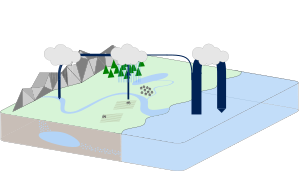
\includegraphics[width=0.8\textwidth]{water_cycle}
\caption{
Illustration of the global hydrological cycle. Water evaporates over the
Oceans and parts of it are transported to the land, where it fills up continental
water storages or re-evaporates.}
\label{fig:introduction:water_cycle}
\end{figure}

On the scale of river basins, the inflow of water through the atmosphere is the
only sustainable source of fresh water \citep{falkenmark04}. Given the competing
water requirements for the production of food, energy, the access to clean water
and the sustaining of ecosystems discussed above, it is clear that water
management is required to minimize conflicts and avoid human suffering. The
management of water resources in turn requires the monitoring and modeling of
the hydrological cycle. Since the fluxes of water in the atmosphere occur across
continental scales, the only currently available way of measuring them is with
the help of satellite observations.

\section{Weather and climate}

Water plays an important role in the weather system. When water evaporates, it
takes up energy from its environment. This energy, the latent heat, is released
when the air cools and the water vapor condensates. The release of latent heat
acts as fuel for the development of vigorous convective storms. The water that
is released by those storms in the form of precipitation can cause flooding and
land slides.

The ability to predict the weather has considerable value for society,
especially for high impact events involving extreme wind speeds or
precipitation. The availability of satellite observations has played an
important role in the steady improvement of weather forecast that occurred
during the last three decades
\citep{bauer15}. Weather forecasting  systems use satellite data to
determine a best estimate of the current state of the atmosphere, which is then
evolved into the future to predict the weather. While most advanced forecasting
systems ingest satellite observations directly and are thus not dependent on
satellite retrievals \citep{bauer10}, their use for improving model
initialization for short-range forecasts is still being investigated
\citep{dehaan14, benjamin21}. Besides that, retrievals of precipitation and
cloud properties are used by weather forecasters to gain situational awareness
and assess potential weather hazards.

%Despite the progress of the last decades, weather forecasts still struggle to
%produce accurate forecasts for specific meteorological contexts
%\citep{schafler18}. In many of those, the misrepresentation of the
%interaction of latent heat release through condensation and the large scale
%dynamics of the atmosphere were found \citep{rodwell13} to play a role.
%Improving the forecasts requires improving the representation of these processes
%in the model, which is where satellite-derived measurements of precipitation and
%clouds can help researchers better understand them.

Water is also an important actor in the climate system. It affects the Earth's
energy budget in multiple ways. Water vapor is the most potent greenhouse gas
and thus contributes strongly to the retention of radiative energy emitted from
the Earth's surface. In the form of clouds, water both cools the Earth system
through the reflection of solar radiation and warms it through the absorption of
upwelling longwave radiation. Although the global effect of clouds is a
pronounced cooling, the effect varies regionally and with the properties of the
clouds. Evaporation and transpiration are important for the transfer of heat
from the Earth's surface to the atmosphere. Since, on average, these two processes
have to be balanced by precipitation, the energy budget of the Earth is directly
linked to precipitation \citep{trenberth09}.

Instead of a passive tracer of atmospheric dynamics, the hydrological cycle must
thus be considered an active component of the both the weather and the climate
system. Both climate science and meteorology therefore rely on satellite observations
of the hydrological cycle to improve their understanding of the Earth system.


\section{A warmer planet}

As a consequence of anthropogenic emissions of carbon dioxide, the Earth's
 climate is heating up. As the Earth system adapts to the increased radiative
 forcing from greenhouse gases, its climate changes. These changes are not
 uniform but vary regionally and across spatial scales. Reliably regional
 predictions of climate change are required to help societies adapt to the
 changing climate. However, our current understanding as well us our ability to
 predict changes at regional scales remains severely limited.

Together with the climate, also the hydrological cycle is changing: Increased
evaporation leads to more frequent droughts at the same time as global
precipitation is expected to increase. Extreme precipitation events are
strengthening and becoming more frequent. The prediction of changes in the
hydrological cycle is complicated by their regional and scale dependence. At the
scales of individual precipitation systems, precipitation increases with the
capacity of warmer air to carry water vapor. Globally, however,
evapotranspiration and thus also precipitation are constrained by the Earth's
energy budget, which limits increases in global precipitation to a lower rate
than that of individual storms\citep{collins13}. These contrasting changes are
in turn modulated by changes in the general circulation, which ultimately
defines the global distribution of precipitation. Moreover, the detection and
prediction of these changes is difficult because on short time scales it likely
to be masked by the internal variability of precipitation.

As part of the hydrological cycle, clouds will change with the climate. Since
cloud reflect incoming solar radiation and the absorb outgoing long-wave
radiation, these changes act as a feed back on the Earth's energy budget and
will thus influence the response of the climate system to increased CO$_2$
concentrations. Whether an individual cloud exerts a net warming or cooling
effect on the climate system depends on its properties such as altitude and
composition as well as its location. The representation of clouds remains an
important challenge for climate models and uncertainties in cloud feedbacks
remain the primary source of uncertainty in predictions of the climate response
to increased CO$_2$ concentrations in the atmosphere \citep{zelinka20}.

Our understanding of climate change has progressed immensely during the last
decade but remains insufficient to make confident predictions at regional
scales. Such predictions are necessary for efficient climate change adaptation.
Satellite observations are therefore essential for improving and validating
climate models as well as the monitoring of changes in the climate system.


\section{Why satellites?}

Considering the importance of rain for a large range of human activities, it is
not surprising that humans have been measuring precipitation and trying to
improve their understanding of the weather system. The most direct and arguably
intuitive way to measure precipitation is through the use of \textit{rain
gauges}. A rain gauge consists of a cavity, which captures rain and from which
the accumulated precipitation can be measured. First records of gauge
measurements of rain date back to as long as 400 years
BC \citep{strangeways2000}. Today, gauge measurements are available from all
continents, however their density varies from country to country and is
oftentimes tied to the local population density.

The main disadvantage of rain gauges is the highly localized character of their
measurements, which limits their ability to accurately capture the spatial
structure of precipitation on short time scales. Moreover, because these
measurements are performed by a large number of public and private actors across
the globe, not all of them are easily accessible for scientists. Effectively,
only $\SI{1}{\percent}$ of the surface of the Earth is estimated to be within a
distance of $\SI{5}{\kilo \meter}$ from the nearest gauge
measurement \citep{kidd17}.

Over land, another important technique for measuring precipitation are
ground-based radars. These radars send out beams of radiation, which are
reflected by rain and snow. Precipitation within a radius several hundreds of
kilometers form the radar can be detected by measuring the amount of radiation
reflected back to the radar. Over land, ground-based radars play an important
role for real-time monitoring of precipitation. However, due to their high
installation and maintenance costs, their spatial availability is irregular and
typically tied to the local population density. In addition to that, the
availability and accuracy of radar measurements may be hampered by complex
terrain as well as the distance from the radar location, which limits the
usefulness of these observations for climatological applications.

The relevance of clouds and precipitation for the hydrological cycle has been
known since before the times of Aristotle \citep{frisinger72}. Nonetheless, the
systematic study of clouds has long remained a secondary focus of modern
meteorology and it took until the 1970s before the importance of interactions
between clouds, weather and climate put them at the forefront of atmospheric and
climate research \citep{stephens03}. Traditionally, cloud observations were
conducted as parts of routine meteorological observations performed on land and
ships \citep{hughes84}. However, these observations were mostly qualitative in
nature indicating only the presence of clouds, a cloud class and their rough
height.

The principal drawback of all of the measurement techniques discussed above is
their limited and irregular spatial coverage. This limits their value for the
monitoring of weather and climate. Satellites have the ability to provide
observations across global scales at high temporal resolutions. Because of this
they ideally complement ground based measurements and have become an essential
source of information for a wide range of scientific, economic and societal
activities.



\chapter{Satellite remote sensing of clouds and precipitation}

The remote sensing of any atmospheric component is based on its interaction with
electromagnetic radiation. By inverting this interaction, the measured radiation
can be used to infer certain properties of that component. This chapter presents
the physical processes, which enable satellites to sense clouds and
precipitation as well as the practical aspects of observing the
atmosphere from space.


The first part of this chapter provides a brief introduction to
radiative transfer (RT) theory, which can be used to describe  the
interaction of radiation with the atmosphere. Based on this, the
principal characteristics of observations across the electromagnetic
spectrum and their sensitivity to hydrometeors%
\footnote{%
Hydrometeor is the collective term for the liquid and frozen particles that
that make up clouds and precipitation.
}%
 are discussed. The remaining part of this chapter then provides an overview of
 the types of satellite observations that were used in the retrieval
 applications that were developed as part of this thesis.
The presentation focuses on observations measuring radiation that is
emitted from the sun or the Earth and its atmosphere, so called
\textit{passive observations}.
%to the electromagnetic radiation measured by satellites. This is
%followed by a discussion of the different types of satellite observations
%relevant to this thesis and their characteristics.


%Doing so, requires a quantitative model of the propagation of radiation through
%the atmosphere. Such a model is provided by the physical theory of 
%Since radiative transfer theory is fundamental to atmospheric remote sensing ,
%this section provides an introduction to radiative transfer in the atmosphere.
%The focus is put on the interaction of radiation with hydrometeors. This
%presentation is mostly based on the more comprehensive texts by Mishchenko et
%al. (2002), Thomas and Stamnes (2002), and Wallace and Hobbs (2006).


\section{Radiative transfer theory}

Radiative transfer theory describes the propagation of a perfectly monochromatic
beam of light through a medium. As this beam propagates through the medium it
interacts with it through electromagnetic and quantum mechanical processes.
Radiative transfer theory provides a simplified model of these interactions,
which is well suited for the conditions of passive remote sensing of the
atmosphere.  The following presentation is  based on the more
comprehensive texts by \citet{mishenko02}, \citet{thomas02} and \citet{wallace06}.
%al. (2002), Thomas and Stamnes (2002), and Wallace and Hobbs (2006).

Electromagnetic sensors measure the mean total energy that is transferred by
electromagnetic radiation over a finite time interval. The way in which this
energy is distributed across the components of the electric field is defined as
its \textit{polarization state}. Mathematically, the polarization state of the
beam can be described using the four dimensional Stokes vector
\begin{align}
  \bm{I} &= \left [ \begin{array}{c}
    I \\
    Q \\
    U \\
    V \\
    \end{array} \right ]
\end{align}
The components $I, Q, U$ and $V$ are called the Stokes parameters and have the
unit of monochromatic energy flux per solid angle. The Stokes vector fully
describes the state of a monochromatic beam of radiation to the extent that it
can be measured by an electromagnetic sensor. Thus any electromagnetic
measurement can be derived from knowledge of the Stokes vector at the position
and orientation of the sensor. Radiative transfer theory describes how the
Stokes vector changes as it propagates through a medium.

\subsection{Interactions with matter}

Radiative transfer theory distinguishes three fundamental processes through
which matter interacts with radiation. These are the emission of
electromagnetic radiation, its absorption and scattering.

\subsubsection{Emission}

At temperatures above absolute zero, all matter emits thermal radiation. Thermal
radiation is produced when matter transitions from a quantum mechanical state
of higher energy to one of lower energy causing the excess energy to be emitted
in the form of radiation. The amount of radiation of a given frequency $\nu$
emitted by a body depends on its temperature and material. It is typically
modeled using a material-dependent emissivity vector $\vec{e}$, which relates
the emission of the material to that of an ideal black body, i. e. a material
that absorbs all incoming radiation:
 \begin{align}
   \label{eq:emissivity}
   \vec{I} &= (\vec{e} \cdot ds) B(T, \nu)
 \end{align}
 Here $B(T, \nu)$ is the radiation emitted by a black body at temperature $T$
 and frequency $\nu$, which is described by Planck's law
 \begin{align}
   B(T, \nu) &= \frac{2 \nu^2}{c^2}\frac{h\nu}{e^{\frac{h\nu}{k T}} - 1},
 \end{align}
 with $c$ is the speed of light in vacuum, $h$  the Planck constant and $k$
 the Boltzmann constant.

 The emissivity is a material property of the medium through which the beam
 propagates and depends on its quantum mechanical properties as well as the
 wavelength of the radiation. The emissivity vector defined above is a
 differential quantity that describes emission from a volume element along an
 infinitesimal step of the propagation path of the beam.


%For a material that is opaque, there is no need to integrate over the full
%volume, since only its surface will contribute to the observed emission.
%The emissivity of a surface can be described using an emissivity vector
%$\vec{e}$ in the same way as for emission from a volume, with the difference
%that its components are unitless and integration over the propagation path is
%not required.

\subsubsection{Absorption}

Absorption refers to the process of radiation being converted into internal
energy of the matter it interacts with. Mathematically, this process is
described by the absorption vector $\vec{\alpha}$, defined as the fraction of
the incoming radiation that is absorbed along an infinitesimal distance $ds$
along the propagation path:
\begin{align}
\vec{I}_\text{absorbed} &= (\vec{\alpha} \cdot\ ds) \odot \vec{I}
\end{align}
Here $\odot$ denotes the element-wise product of the absorption vector and
the Stokes vector $\vec{I}$ of the incoming radiation. Absorption may be
understood as the inverse process of thermal emission. Formally, this is
expressed by Kirhoff's  law of radiation
\begin{align}
  \vec{\alpha} &= \vec{\epsilon},
\end{align}
which states that the absorption vector is identical to the emissivity vector
defined in Eq.~\ref{eq:emissivity}. This law is applicable to all matter in the
atmosphere given that it is in a state of local thermal equilibrium (LTE). LTE
occurs when the density of matter is sufficiently high so that the population
rates of energy states above the ground state are determined by thermal
collisions rather than the absorption of radiation. This decouples the emission
of radiation from the radiation field itself, allowing the simplified treatment
of matter as thermal emitters with the emission rates independent of the
radiation field. LTE is a valid assumption for radiative transfer in the
troposphere.

\subsubsection{Scattering}

Scattering describes the effect that inhomogeneities of the medium have on the
propagation of the beam. When a plane-parallel electromagnetic wave encounters
such inhomogeneities, it is scattered in all directions. Mathematically, the
scattering of a beam of light propagating in direction $\vec{n}$ into the
direction $\vec{\hat{n}}$ is described by the phase matrix
$\mat{Z}(\vec{\hat{n}}, \vec{n})$:
\begin{align}
  \vec{I}_\text{scattered}(\vec{\hat{n}}) &= \mat{Z}(\vec{\hat{n}}, \vec{n}) \vec{I}(\vec{n})
\end{align}
Since parts of the energy flux of the beam are deviated from the direction of
propagation, the intensity of the radiation along the beam is decreased. As it
propagates through the medium, the intensity of a beam is thus decreased by the
effects of absorption and scattering. The combination of these two processes is
referred to as \textit{attenuation} or \textit{extinction} and is described by
the attenuation matrix $\mat{K}$, which is the sum of the absorption vector
$\vec{\alpha}$ and the fraction of radiation scattered away from the propagation
path:
\newcommand*{\vertbar}{\rule[-1ex]{0.5pt}{2.5ex}}
\newcommand*{\horzbar}{\rule[.5ex]{2.5ex}{0.5pt}}
\begin{align}
  \vec{K} &=
  \left [ \begin{array}{cccc}
      \vertbar & \vertbar & \vertbar & \vertbar \\
      \vec{\alpha} & \vec{0} & \vec{0} & \vec{0} \\
      \vertbar & \vertbar & \vertbar & \vertbar
    \end{array} \right ]
       + \int_{\vec{\hat{n}}} d\vec{\hat{n}}\ \mat{Z}(\vec{\hat{n}}, \vec{n})
\end{align}

The strength of the scattering interaction depends on the relation of the size
of the inhomogeneities and the wavelength of the radiation. When the scale of
inhomogeneities is much smaller than the wavelength, the effects of scattering
can often be neglected. As the size of the inhomogeneities increases, the
strengths of the scattering increases and scattering effects must be taken into
account. The scattering interaction drastically complicates calculating the
evolution of the radiation because it requires taking into account the radiation
that is scattered into the line of sight from all directions. Because of their
relatively large size, scattering effects of hydrometeors need to be taken into
account across most of the electromagnetic spectrum. Simulations of radiative
transfer that involve hydrometeors are therefore more complex to perform than
those that don't.


\subsection{The radiative transfer equation}

The previous section introduced the fundamental interactions of radiation
with matter and how they are described mathematically in radiative transfer
theory. Combining the three processes of emission, absorption and scattering,
the change that a beam undergoes as it travels a distance $ds$ along its
propagation path through the atmosphere is described the vector radiative
transfer equation (VRTE):
\begin{align}\label{eq:vrte}
  \frac{d\vec{I}(\vec{n})}{ds} &=
  -\mat{K}\vec{I}(\vec{n}) + \vec{\alpha} \cdot B_\nu(T) + \int_{\hat{\vec{n}}} d\hat{\vec{n}} \ \mathbf{Z}(\vec{n}, \vec{\hat{n}}) \vec{I}(\vec{\hat{n}}).
  \end{align}

The first term on the right hand side is the extinction term, which represents
the combined effects of absorption and scattering of radiation out of the
propagation direction, which act to decrease the intensity of the radiation
along the line of sight. The second term represents emission along the line of
propagation, with the emissivity vector $\bm{\epsilon}$ replaced by the
absorption vector $\bm{a}$ according to Kirchoff's law of thermal radiation.
The third term represents the radiation that is scattered into the line of
sight. Both of these terms act to increase the intensity of the beam. 

\section{Observations of hydrometeors}
%
\begin{figure}[!tbp]
  \centering
  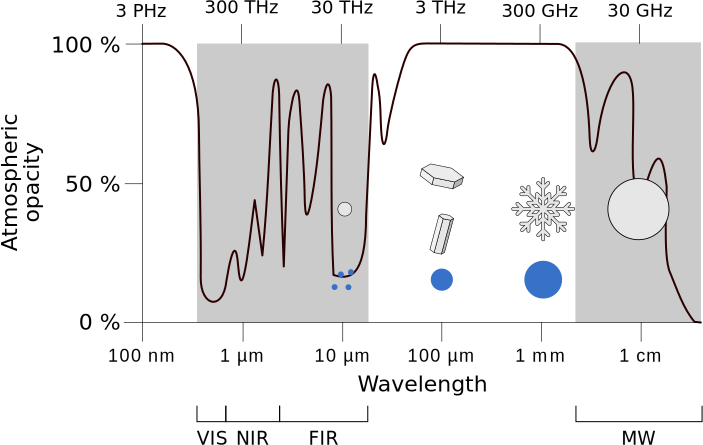
\includegraphics[width=0.75\textwidth]{spectrum}
  \caption{Overview of the electromagnetic spectrum used for hydrometeor retrievals. The black
    curve shows the variation of the atmospheric opacity across the spectrum.}
  \label{fig:radiative_transfer:spectrum}
\end{figure}

Radiative transfer theory describes the propagation of radiation through the
atmosphere in terms of its radiative properties, which are represented by the
absorption vector $\vec{\alpha}$, the extinction matrix $\vec{K}$ and the phase
matrix $\vec{Z}$. In order to apply radiative transfer theory to gain an
understanding of remote sensing observations of the atmosphere, the gases,
aerosols and hydrometeors contained in it must be related to its radiative
properties.

The radiative properties of the atmosphere are strongly dependent on the
wavelength $\lambda$ at which it is observed. The applications presented in this
thesis focus on observations from the visible (VIS,
$\SI{350}{\nano \meter} \leq \lambda < \SI{720}{\nano \meter}$), infrared (IR,
$\SI{0.72}{\micro \meter} \leq \lambda < \SI{20}{\micro \meter}$), and microwave
(MW, $\SI{1}{\milli \meter} \leq \lambda < \SI{1}{\meter}$) regions, which
encompass most commonly used wavelength for the remote sensing of clouds and
precipitation.

An overview these regions within spectrum of electromagnetic radiation is
provided in Fig.~\ref{fig:radiative_transfer:spectrum}. The graph provides an
approximate depiction of the atmospheric opacity in the absence of hydrometeors.
When viewed from a satellite, the atmospheric opacity gives an indication of how
far down into the atmosphere a sensor can 'see'. Generally, where the opacity is
low, the satellite can see down to the surface, while where it is high it is
sensitive only to the upper parts of the atmosphere.

Observations of the atmosphere are the results of the combined effects of gases,
aerosols and hydrometeors in the atmosphere. To gain an understanding of the
information that certain observations provide on hydrometeors, it is helpful to
decompose the contributions into a clear-sky component, which takes into account
only the effects of molecules aerosols, and a cloudy-sky component, which takes
into account the effects of hydrometeors. As a first approximation, the clear-sky
component maybe viewed as the background upon which the hydrometeors are
observed.

\subsection{The atmospheric background}

Observations at short wavelengths differ from those at long wavelengths with
respect the source of the observed radiation. At wavelengths in the visible and
near infrared regions, the largest part of the observed radiation stems from the
sun. This is because, at these short wavelengths, black body radiation at
typical atmospheric temperatures is small compared to reflection of solar
radiation. As the wavelength increases, the intensity of solar radiation decreases
while that of a black bodies at atmospheric temperatures increases. At wavelengths
exceeding $\approx \SI{3}{\micro \meter}$, emission from atmospheric constituents
dominates the intensity of reflected solar radiation. This threshold separates
the thermal ($\lambda \geq \SI{3}{\micro \meter}$) from the near infrared. At
these wavelengths solar emission can generally be neglected and all observed
radiation originates from the atmosphere itself or the Earth's surface.

The atmospheric opacity displayed in Fig.~\ref{fig:radiative_transfer:spectrum}
corresponds to the combined effects of absorption and extinction by gases in the
atmosphere. Gases affect radiation mostly through absorption and emission, while
scattering plays a role only in the visible range. The reason for this is the
small size of the molecules (around $\SI{1}{\nano \meter}$) compared to the
wavelengths of the radiation.

There is little absorption in the visible range with most of it due to water
vapor. In the near and thermal infrared, absorption increases but is concentrated
in discrete absorption bands, which makes the opacity of atmosphere highly
variable across wavelengths. The principal gaseous absorbers in the infrared
region are water vapor, cabon dioxide and ozone. Absorption also plays an
important role in the microwave region with significant contributions from water
vapor, oxygen, nitrogen and ozone. 

In addition to the effects of gases, satellite observations can be affected by
the presence of aerosols. Aerosols are larger than gas molecules but their
scattering and absorption effects remain mostly limited to the VIS and NIR
regions. At longer wavelength, aerosols have no significant effect on the
observations.

\subsection{Physical and radiative properties of hydrometeors}

The radiative properties of hydrometeors depend on their size and whether they
are in the liquid or frozen phase. Because the dielectric properties of ice and
water differ significantly across the electromagnetic spectrum, hydrometeors of
similar sizes have drastically different radiative properties in certain
wavelength domains. To provide an overview of the sizes of the principal classes
of hydrometeors with respect to the wavelengths of the electromagnetic spectrum,
they are displayed in Fig.~\ref{fig:radiative_transfer:spectrum} at the
wavelengths corresponding to their approximate sizes. Liquid hydrometeors are
identified using blue coloring, while white corresponds to frozen hydrometeors.

Among the smallest hydrometeors are liquid cloud droplets with typical sizes
around $\SI{5}{\micro \meter}$. At sizes of around $\SI{25}{\micro \meter}$,
water drops become large enough to fall out of the clouds. Small, precipitating
liquid droplets that range in size from $25 to \SI{250}{\micro \meter}$ are
referred to as drizzle. Larger drops are classified as rain. Typical sizes of
rain drops are around $\SI{1}{\milli \meter}$ but can become as large as
$\SI{5}{\milli \meter}$.

At temperatures below $\SI{0}{\celsius}$ ice crystals can form in the
atmosphere. Their sizes range from $\SI{1}{\micro \meter}$ to
$\SI{1.5}{\milli \meter}$ with typical sizes around $\SI{100}{\micro \meter}$.
Snow flakes are aggregates, which form through the collision of ice crystals.
These range in size from hundreds of micrometers millimeters to several
centimeters.

When snowflakes collide with liquid drops at temperatures below
$\SI{0}{\celsius}$, the liquid drop freezes upon the snowflake causing it to
grow. This process is called riming. Heavily rimed snowflakes are referred to as
graupel and have typical sizes of around $\SI{1}{\centi \meter}$. Finally, the
largest hydrometeors are hailstones, which form only in strong thunderstorms and
can reach sizes of up to $\SI{10}{\centi \meter}$$.


%Most observations of clouds are affected not only by the clouds themselves but
%also by other constituents of the atmosphere. In the following, we will
%therefore first discuss observations without clouds, so called \textit{clear
%  sky} observations, as these form the background for the observations of
%hydrometeors. This is followed by a discussion of the observable effects of
%hydrometeors on the observations, which gives rise to the signal in the
%\textit{all-sky observations} that can be used to infer the physical properties
%of hydrometeors.

%\subsection{The Earth's surface}
%
%The characteristics of the Earth's surface vary considerably across the
%electromagnetic spectrum. In the visible range, the surface absorbs large parts
%of the radation. The darkest surfaces are the ocean which absorbs around
%$\SI{95}{\percent}$ of the incoming radiation. Bare land surface and forests are
%considerable brighter but still absorb most ($\approx \SI{75}{\percent}$) of the
%incoming radiation. In contrast to that, snow and ice covered surface reflect
%nearly all of the incoming radiation and thus appear very bright.
%
%In the infrared region of the electromagnetic spectrum the emissivity of the Earth surface
%increases significantly. For wavelengths between $3$ and $\SI{20}{\micro \meter}$ the emissivity
%of most surface types is larger than $0.9$. At these wavelengths the surface is very effective at
%emitting and absorbing radiation and there is little contrast between different surface types.
%
%In the microwave region surface emissivity patterns are more complex. Emissivity
%from land is relatively high, while emissivity from water surfaces is low. The
%contrast between land and surface increases with the wavelength. Emissivities
%from snow and ice are lower than that of most bare land surface but higher than
%that of water. The emissivity furthermore depends on the viewing angle and the
%polarization of the radiation.
%
%While these general tendencies are helpful for a qualitative analysis of
%satellite imagery, it should be noted that they only provide a rough
%characterization of the behavior of the Earth's surface across the
%electromagnetic spectrum. Accurate, quantitative modeling of surface
%emissivities is still an unsolved problem and thus remains an area of
%active research.

\subsection{Cloudy sky}

Due to their comparably large sizes, the scattering effects of hydrometeors need
to be taken into account across most wavelengths from the VIS to the MW regions.
In the VIS and NIR there is little absorption from either water or ice.
Hydrometeors thus mostly deviate radiation from its propagation path without
significantly decreasing its intensity. Clouds observed at these wavelengths
typically appear bright because the solar radiation scattered back towards
the sensor is much more intense than reflection from the surface.

In the FIR region, both water and ice are strongly absorbing. Because the
ambient temperature decreases with altitude in the troposphere, opaque clouds
emit less intense radiation than the surface or water vapor below them.
At wavelength at which there is weak absorption from water vapor, so called
\textit{window channels}, radiation from opaque clouds can be used to
infer the temperature at the cloud top, which is related to the altitude of
the cloud.

At microwave frequencies, liquid water is a much more efficient absorber than
ice. Furthermore, for passive observations the scattering from hydrometeors at
frequencies below $\SI{50}{\giga \hertz}$ can be neglected. The principal
interaction with hydrometeors at these wavelength is therefore thermal emission
and absorption from liquid cloud droplets and precipitation. Since water
surfaces have low emissivities at these wavelengths, emission from liquid
hydrometeors causes a distinct signal in the observations.

At frequencies above $\SI{50}{\giga \hertz}$, passive microwave observations
become sensitive to the scattering from large snow flakes. This scattering
signal is important for sensing precipitation over land, where the emission
signature from liquid hydrometeors may not be detectable due to the much warmer
background surface.

\section{Satellite observations}

The information content of satellite observations on hydrometeors is strongly
dependent on the wavelength of the radiation. Because radiation at different
wavelengths is sensitive to different properties and types of hydrometeors, 
observations at different wavelength provide complementary information on
them. In addition to the wavelength, other characteristics of the observations
such as temporal and spatial resolution determine how well different satellite
observations can be used to characterize hydrometeors from space.

Due to the technical complexity of operating specialized sensors in space, the
availability of observations and their characteristics are ultimately determined
by a trade-off between technical and financial constraints on the one side and
scientific value on the other. Since there is only a very limited number of
satellite mission dedicated specifically to observations of hydrometeors,
leveraging the full potential of available satellite imagery requires exploiting
and combining a wide range of observations of different types.

\subsection{Sensor types}

The above discussion of radiative transfer in the atmosphere focused on
observations of radiation that originates either from the sun or the Earth and
its atmosphere. Sensors that measure these types of radiation are called passive
sensors because they do not emit any radiation themselves. \textit{Active
sensors}, on the other hand, emit radiation and measure how much of that
radiation is scattered back to the sensor. The active sensors that are used for
the remote sensing of hydrometeors are mainly radars and lidars. These sensors
measure the time of travel between emission and reflection, which can be used to
infer the distance from the detector in addition to the intensity of the
reflected radiation. This allows them to profile the atmosphere along the line
of sight, leading to much higher vertical resolution than what can be obtained
with passive sensors.

From an observational perspective, the principal difference between radars and
lidars are the wavelengths at which they operate. Lidars employ radiation with
relatively short wavelengths, which makes them sensitive to very small
hydrometeors as well as molecules and aerosols in the atmosphere. In contrast to
that, radars operate at MW wavelengths, which makes the sensitive only to
hydrometeors. In general, active sensors are much more sensitive to the
scattering from small particles than their passive counterparts because of the
intensity of the emitted beam.

\subsection{Resolution and coverage}

In addition to the information content that observations can provide on
hydrometeors, their ability to resolve spatial and temporal variability as well
as how much of the globe they cover are important characteristics, which
influence their suitability for different applications.

The orbit in which a satellite is placed plays an important role in determining
these characteristics. For earth observations, two principal classes of orbits
can be distinguished: Geostationary and low-earth orbits. Satellites in
geostationary orbit rotate around the Earth at the same angular velocity as the
Earth rotates around its axis. This allows them to hover over the same position
on the Earth's surface. Since the field of view of the satellite is constant it
can provide observations with high temporal resolution at all locations below
the satellite. This makes these satellite suitable for many near real-time
applications in weather forecasting.

The disadvantage of geostationary platforms is their long distance from the
Earth, which is around $36\ \SI{000}{\kilo \meter}$. Since the spatial
resolution of microwave sensors is limited by the long wavelengths of the
radiation, they are currently not deployed on these platforms. Geostationary
therefore typically carry VIS and IR sensors, which can produce observations
at very high spatial resolutions. Besides that, geostationary satellites
are always located over or close to the locator. The resulting viewing geometry
causes their resolution to degrade at high latitudes.

A common type of low-Earth orbit used for Earth observing satellites are polar
orbits in which the satellite passes above or nearly above the poles. The
rotation of the Earth between consecutive orbits allows these satellites to
achieve global coverage. The low altitude of these orbits ($300
- \SI{1000}{\kilo \meter}$) makes them suitable also for microwave sensors but
decreases the spatial coverage of the sensor. The swaths of sensors in low-earth
orbits are typically limited to a few thousand kilometers in width. Depending on
the exact size of the field of view and the location on Earth, the time between
consecutive overpasses for a fixed position can be as high as $\SI{12}{\hour}.

Fig.~\ref{fig:remote_sensing:viewing_geometries} shows the field of views of
the Advanced Baseline Imager on the GOES 16 geostationary satellite and the
GPM Microwave Imager on the polar-orbiting GPM Core Observatory. The observations
from both satellites are projected onto the corresponding location on the Earth.
This illustration clearly shows the differences that the satellite orbit makes
for the observations. While the geostationary satellite can permanently observe
a large part of the hemisphere below it, the polar orbiting satellite sees only
a comparably thin stripe of the globe.

\begin{figure}[!hbpt]
  \centering
  \includegraphics[width=0.8\textwidth]{viewing_geometries}
  \caption{Viewing geometries of geostationary and polar-orbiting satellites
  drawn to scale. The illustration shows geo-located satellite observations from
  the GOES 16 geostationary satellite in purple and from the polar-orbiting GPM
  Core Observatory in orange. The black spheres mark the instantaneous satellite
  positions.}
  \label{fig:remote_sensing:viewing_geometries}
\end{figure}

\subsection{Example: Satllite observations of Hurricane Ida}

Figure~\ref{fig:radiative_transfer:observations} illustrates the different types
of observations used for the remote sensing of hydrometeors using observations
of Hurricane Ida shortly before landfall on August 30, 2021. The first row of
panels shows observations derived from the Advanced Baseline Imager on the GOES
16 geostationary satellite. Panel (a) shows a natural color composite, which
combines observations from 3 channels from the VIS and NIR to create an image
emulating human color vision. Panel (b) shows observations from the NIR.
Differences in the dielectric constant of water and ice cause ice clouds to
absorb incoming solar radiation much more strongly than water clouds. The high
ice clouds that cover the Hurricane therefore appear much darker than in the RGB
image. Panel (c) shows observation from a window channel in the FIR. Since it is
a window channel, most of the radiation observed in cloud free areas stems from
the Earth's surface and thus appear bright. Where clouds are present the
observed brightness temperatures are closely related to the atmospheric
temperature at the altitude of the cloud and thus colder than the surface.

Panel (c) and (d) show passive microwave observations at $\SI{18.7}{\giga
  \hertz}$ and $\SI{166}{\giga \hertz}$. At the very low microwave frequencies
only the a thermal emission from precipitation in the hurricane is visible over
the cold ocean surface, while the clouds overland yield no signal. At the higher
microwave frequencies, the surface is not visible due to emission from water
vapor. Scattering by snow particles causes a cold scattering signal from the
thickest clouds around the Hurricane.

Finally, panel (e) shows Ku-band radar reflectivities from the GPM
dual-frequency precipitation radar along a vertical cross section of the
Hurricane. The signal in the radar observations is the amount of energy that is
reflected back to the sensor. Due to the relatively low frequency of the
radar, it is only sensitive to large, precipitation hydrometeors.


\begin{figure}
  \centering
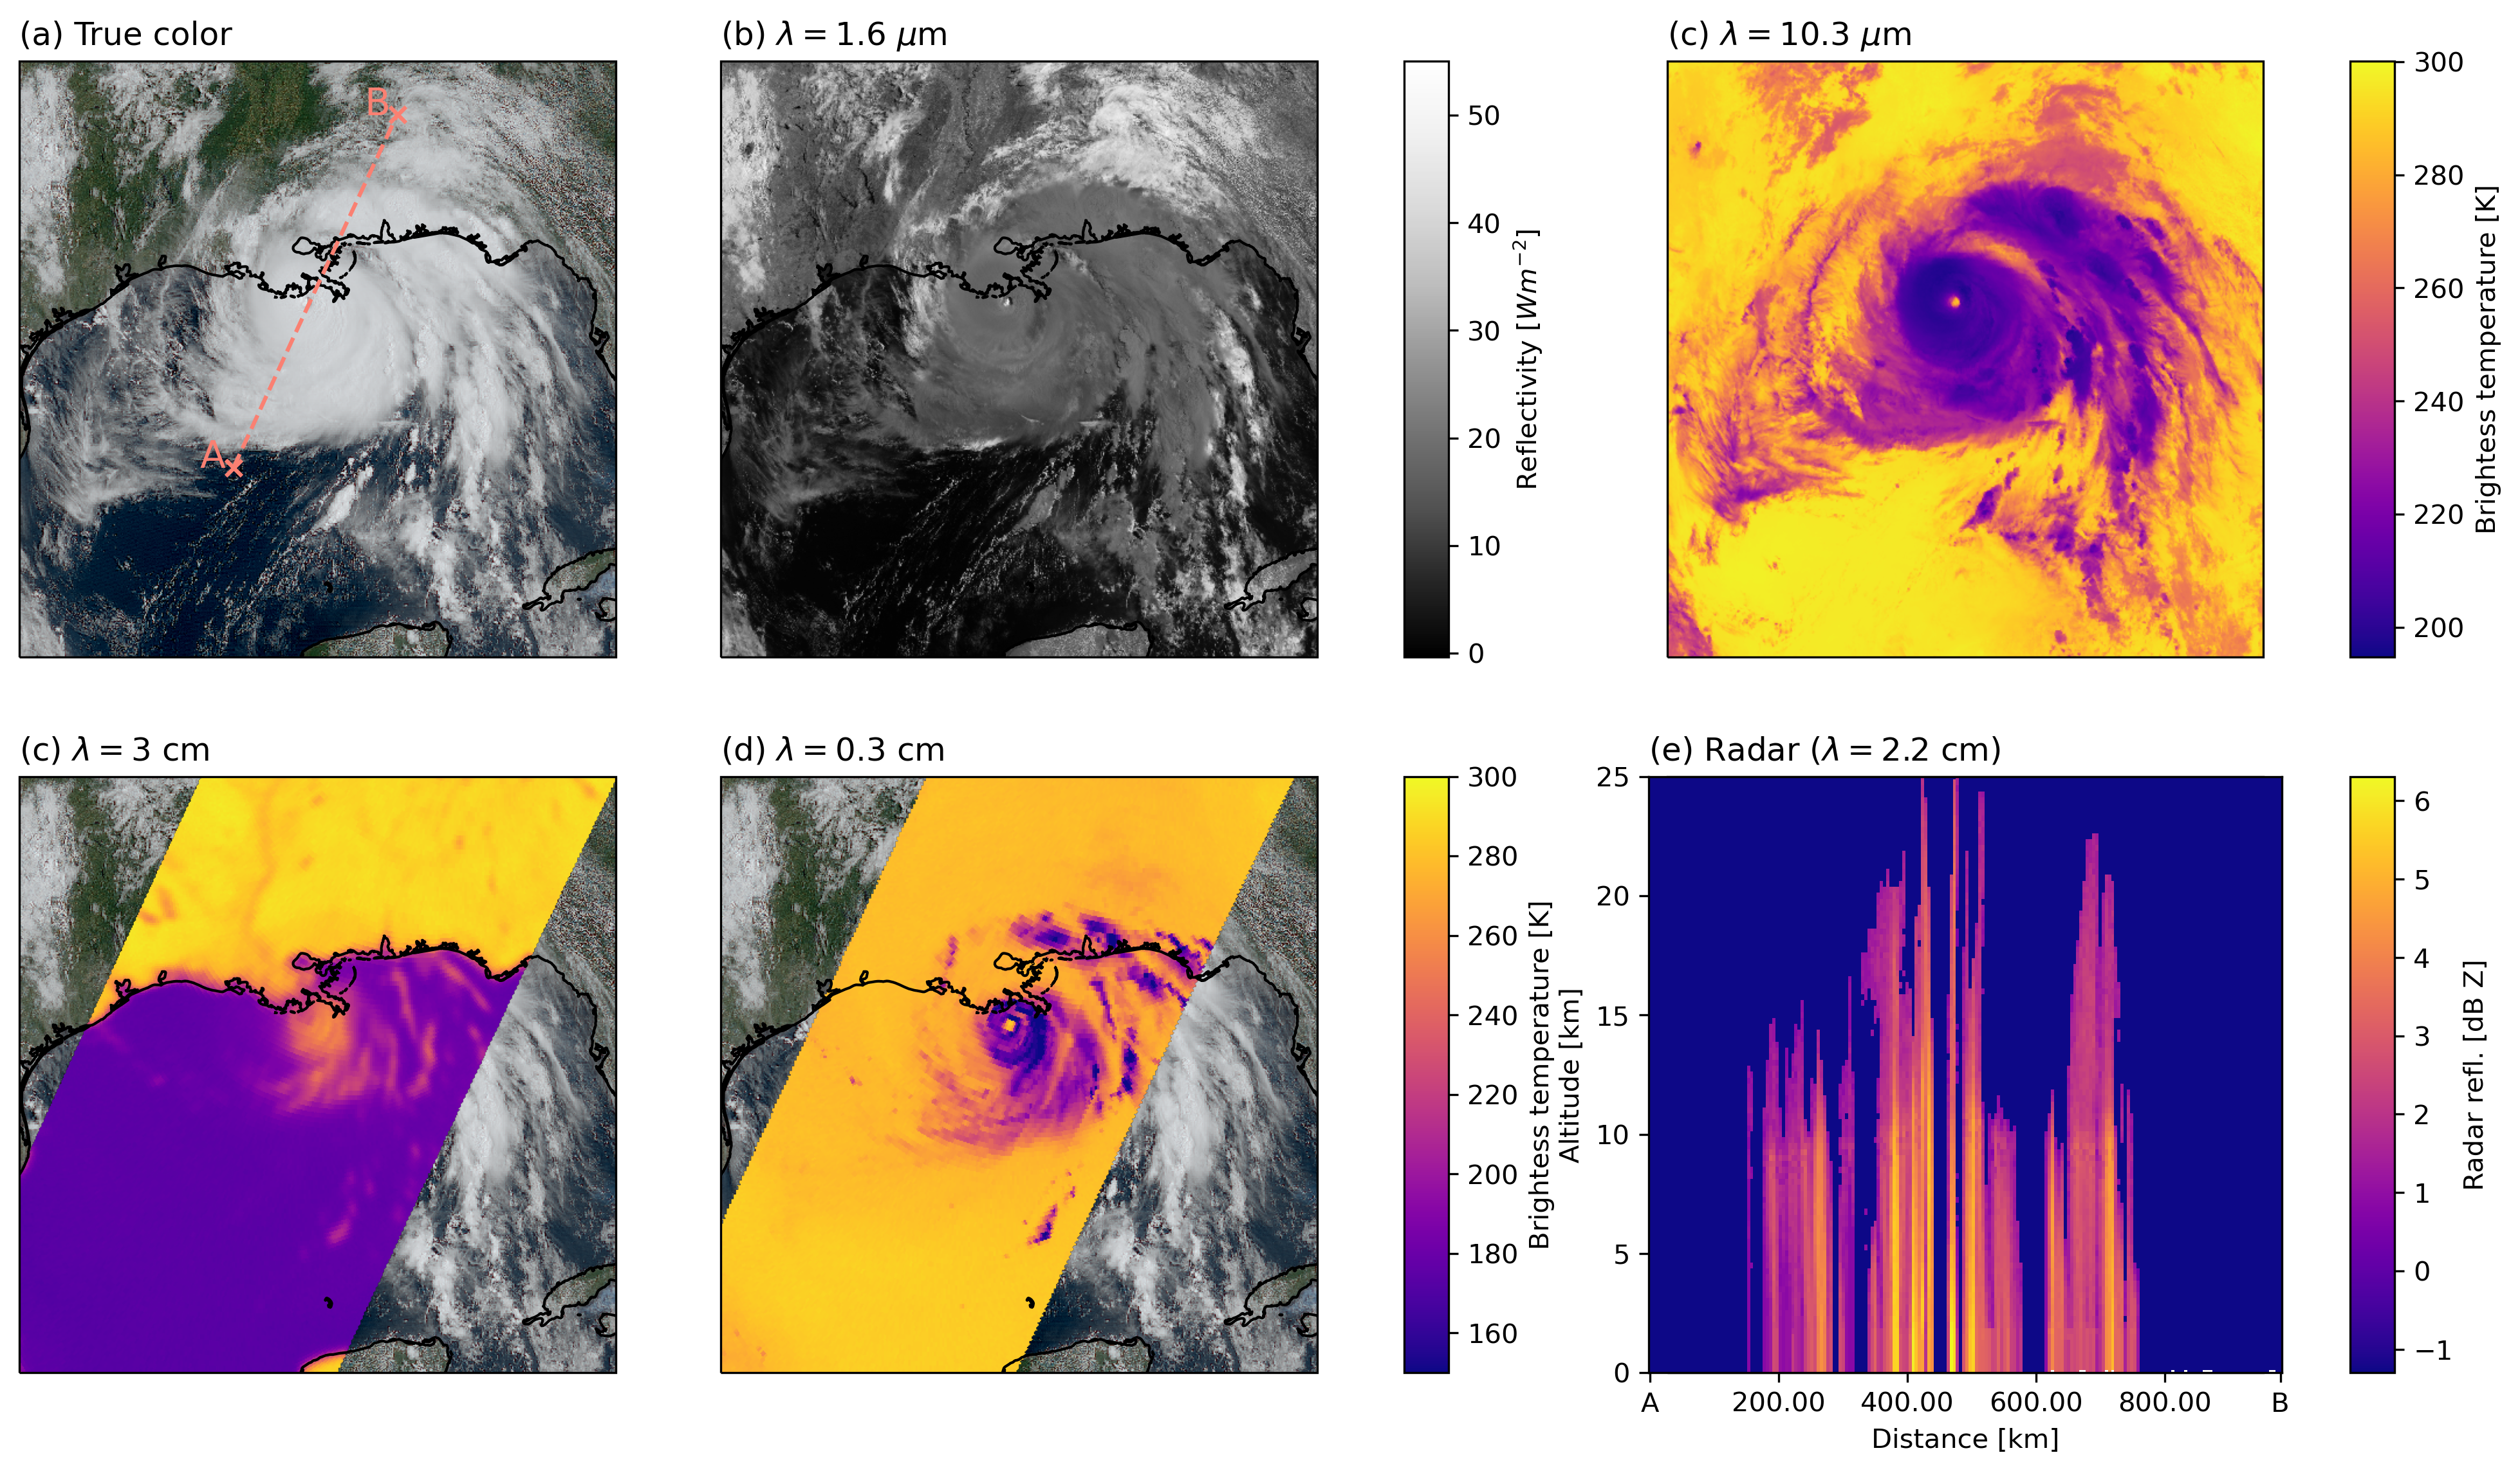
\includegraphics[width=\textwidth]{observations}
\caption{Satellite observations of Hurricane Ida on 2021-08-29 15:09 UTC.
  Panels (a), (b), (c) show observations from the VIS and IR regions obtained
  by the Advanced Baseline Imager on the GOES 16 geostarionary satellite.
  Panels (d) and (e) show passive microwave observations from the GPM microwave
  imager. Panel (f) shows the curtain of radar reflectivity measured by the GPM dual-frequency
  precipitation radar (DPR) along the dashed line shown in panel (a).}
\label{fig:radiative_transfer:observations}
\end{figure}


\chapter{Machine learning for remote sensing retrievals}
Radiative transfer theory describes how radiation that interacts with
hydrometeors produces an electromagnetic signal in satellite observations. Since
the purpose of the observations is to provide information on the physical
properties of hydrometeors, a way must be found to relate the observations to
those properties. This process is referred to as retrieval. This chapter
presents the mathematical formulation of the retrieval problem and provides a
brief introduction to the machine-learning-based methods to solve it.

\section{The retrieval problem}
\label{sec:machine_learning:retrieval_problem}

% So how can these observations be turned
%into estimates of physical properties? This is not a simple task because the
%observations are typically affected by non-negligible measurement noise and,
%more importantly, are generally ambiguous in the sense that physically different
%atmospheric states can produce nearly identical observations.

Mathematically, the problem of determining properties of hydrometeors from
satellite observations can be formulated as finding a state vector%
\footnote{ The notation for the state and observation vectors was deliberately
chosen to be the opposite of the conventions of inverse problem theory to make
it consistent with the conventions used in machine learning. }
$\vec{y} \in \mathrm{R}^{n}$ that describes the physical properties of the atmosphere from a
vector of observations $\vec{x} \in \mathrm{R}^{m}$. This so-called
\textit{retrieval problem} can be solved using the mathematical framework of
inverse problem theory. In inverse problem theory, the underlying assumption is
that the observations $\vec{x}$ are generated by a physical processes, which
can be described using a forward model function $f: \mathrm{R}^n \rightarrow
\mathrm{R}^m$, but may be affected by a random error $\vec{\epsilon} \in
\mathrm{R}^M$:
\begin{align}\label{eq:inverse_problem}
  \vec{x} &= f(\vec{y}) + \vec{\epsilon}
\end{align}

An exact solution to this problem does not exist. Because of the random noise
$\vec{\epsilon}$, the equation can never be strictly satisfied. Furthermore,
there usually exist many states $\vec{y}$ that produce similar measurements
$\vec{x}$, thus rendering the problem underconstrained. Since it does not
admit a unique solution, the retrieval problem is \textit{ill-posed}.

Although an exact solution to the retrieval problem is not possible, Bayesian
statistics provides a framework to extract the available information from the
observations. In the Bayesian approach, both the observations $\vec{x}$ and the
atmospheric state vector $\vec{y}$ are assumed to be random variables.
Furthermore,  it is assumed that $\vec{y}$ is distributed according to a known
\textit{a priori} distribution $p(\vec{y})$. Instead of a single, unique state
$\vec{y}$, the solution of the problem then becomes the \textit{a posteriori} (or
\textit{posterior}) distribution $p(\vec{y} | \vec{x})$ of the atmospheric
state. According to Bayes theorem, the a posteriori distribution for given
observations $\vec{x}$ is given by
\begin{align}\label{eq:bayes}
  p(\vec{y} | \vec{x}) &= \frac{p(\vec{x}|\vec{y})
  p(\vec{y})}{p(\vec{x})}.
\end{align}
Traditionally, Bayesian methods for solving the retrieval problem make use of
the right-hand side of Eq.~\ref{eq:bayes} to approximate the posterior
distribution. The approach pursued in this thesis is to learn the posterior
distributions $p(\vec{y}|\vec{x})$ directly from data. How this can be done is
the topic of the remainder of this chapter.

\section{Machine learning}


The field of machine learning is concerned with the development of algorithms
that can learn to solve computational tasks from data. More specifically, the
methods considered here solve the problem of \textit{supervised learning}. In
supervised learning, the task is to learn how to produce a certain output
$\vec{y}$ from inputs $\vec{x}$ given a set of pairs $\{(x_i, y_i)\}\text{ for
}i = 1, \ldots, N$ of specific input values $\vec{x}_i$ and corresponding output
values $\vec{y}_i$. In general, the inputs $\vec{x}$ and outputs $\vec{y}$ may
represent anything from simple numbers to images or texts. For the applications
considered here, the inputs are typically satellite images, and the outputs are
the corresponding physical quantities to be retrieved.

Machine learning has gone through a wave of immense popularity during the 2010s
triggered by the success of \textit{deep learning} methods in addressing a range
of computational problems in computer vision, natural language processing, and
artificial intelligence. The idea behind deep learning is to construct
increasingly powerful models from a hierarchy of simple models. Given sufficient
data, these models can learn highly complex relationships and require less
guidance from human experts to achieve good performance.

\subsection{Shallow machine learning}

Although the focus of this thesis is deep learning, this section will use a very
shallow model to illustrate the basic principles of machine-learning-based
remote sensing retrievals. The considered example tries to estimate rain at the
surface from infrared (IR) observations at a wavelength of $\lambda =
\SI{10.3}{\micro \meter}$. The training data, which contains of the in- and
outputs from which a solution to the retrieval problem should be learned, is
derived from co-locations of observations from the GOES 16 geostationary
satellite and the combined radar and passive microwave retrievals from the GPM
core observatory (see Sec. \ref{sec:radiative_transfer:synergies}).

The input $x$ for this particular example corresponds to the measured radiation
at a single pixel of the geostationary observations while the output $y$ is
given by the rain rate measured by the GPM core observatory. The retrieval
assumes a linear relationship between the observations $x$ and the rain rate $y$
in order to determine the precipitation corresponding to the geostationary
observations:
\begin{align}
  y &= a x + b
\end{align}
The two parameters of the linear regression model are the slope $a$ and 
the intercept $b$. They can be determined by finding the values that minimize the
squared error between the predictions and the true rain rates.

Panel (a) in Fig.~\ref{fig:machine_learning:linear_regression} shows the
distribution of the training data together with the learned relationship between
input and output data. This view reveals that the relationship is not very
robust, which becomes even clearer when the retrieval results (panel (b)) are
compared to the reference precipitation (panel (c)). The linear regression model
simply predicts rain almost everywhere where there is a cloud but completely
fails to reproduce the structure in the reference precipitation.

\begin{figure}
  \centering
  \includegraphics[width=\textwidth]{linear_regression.png}
  \caption{Example of a very simple precipitation retrieval. Panel (a) shows a
    density plot of the distribution of the input-output pairs, which consist of
    IR brightness temperatures and surface precipitation rates. The white line
    shows the linear relationship between observations and rain rate obtained by
    linear regression. Panel (b) shows retrieved precipitation rates when the
    learned relationship is applied to real observations. Panel (c) shows the
    true precipitation rates as present in the training data. Because of the
    narrow swath of the GPM precipitation radar the precipitation is not known
    across the full scene. }
  \label{fig:machine_learning:linear_regression}
\end{figure}

Given the bad performance of the simple linear regression model, it is natural
to ask how a better-performing model can be found. In general, there are three
dimensions along which a machine learning model can be improved:
\begin{description}
\item[Model expressivity:] The model used in this example can only learn
  linear relationships between input and output. The range of mathematical functions
  that a model can represent is referred to as its \textit{expressivity}. Increasing
  the model expressivity enables it to learn  more complex relationships between
  the input and output.
\item[Amount of input information:] The scatter plot in panel (a) of
  Fig.~\ref{fig:machine_learning:linear_regression} shows that the problem of
  retrieving precipitation from infrared (IR) observations is highly degenerate. For any
  value of the observations, the training data contains a wide range of different precipitation
  values. This makes it impossible to assign a unique `right' precipitation rate
  to an observed brightness temperature. The degeneracy can be decreased by
  adding more information to the input. One way to achieve this, for example, is
  to add observations from other channels or information from neighboring
  pixels. Depending on the problem, this may provide  more flexibility
  to distinguish different precipitation rates to the model.
\item[Amount of data:] A machine learning model can only learn relationships
  that are sufficiently well represented in the training data. For more complex
  retrievals than this one, larger amounts of training data are crucial for good
  retrieval performance.
\end{description}

Traditionally, the difficulty in improving a machine learning model was that it
is not sufficient to just increase the model expressivity or the amount of input
information. Both measures increase the flexibility of the model and may
thus cause it to \textit{overfit}. Overfitting occurs when the
model learns spurious relations from the training data, which are not actually
representative of the true relationship between input and output. This typically
causes predictions on unseen data to deteriorate drastically. Overfitting can be
counteracted by artificially reducing the expressivity of the model, a process
that is called \textit{regularization}, as well as by increasing the amount of data
that is used to train the model. However, the time and computational resources
that are required for training typically increase with the amount of data. If
the  increase is too rapid, the amount of data that a machine learning model
can be trained on may be limited.

Because of this, machine learning models traditionally depend on careful tuning
to the task at hand. Especially the trade-off between model expressivity and the
amount of data that can be used to train it required a multi-disciplinary
approach that combined domain-specific knowledge with machine-learning
experience to develop a good-performing model. A particular difficulty of
shallow models was their inability to handle large inputs with low information
density, such as the pixels from an image. Providing a shallow model with too
many inputs typically makes the models prone to overfitting and more difficult
to train. This gave rise to the practice of \textit{feature engineering}, which
consists of manually designing input variables that encode high-level
information in task-specific input features.

It should be noted that the linear regression model used here is extremely
simple and that there exist shallow machine learning methods that would likely
work much better for this example. Nonetheless, the application is not totally
unrealistic, given that it is similar to early precipitation retrievals from
geostationary observations \citep{vicente98}. To overcome the limitations of the
linear regression, the model from \citet{vicente98} predicts precipitation in
log-space and uses weather model data to post-process the retrieval results.
Modified versions of this retrieval are still in operational use today
\citep{siqueira19}.

\subsection{Deep learning}

The example discussed above illustrated the limitations of very shallow machine
learning methods that deep learning aims to overcome. The essential promise of
deep learning is that it decouples the dimensions along which a machine learning
model can be improved. Deep learning models achieve high expressivity by
stacking a large number of simple models and maximizing the amount of input
data. Since the training time of deep learning methods scales linearly with the
amount of available data while the required memory remains constant, the
increased model expressivity can be balanced with large amounts of training
data. This enables deep learning models to learn highly complex relationships
from data without the risk of overfitting.

  \subsection{Neural networks}

  Seen from a more general perspective, the linear regression model considered
  above is just a transformation from the input $x$ into the output $y$ with a
  set of learnable parameters, in this case, the slope and intercept of the
  regression. A neural network is just a sequence of such parametrized
  transformations, which are referred to as \textit{layers}. Each layer
  transforms an input vector into an output vector, which is passed on to the
  next layer. The exact form of each transformation can be adapted through its
  parameters, which is done by minimizing an error metric over the training
  data.

  Defined in this way, every neural network also satisfies the definition of a
  layer. This allows any neural network to be used as a component within a
  larger network.

  %sAn important characteristic of this definition of a neural network is its
  %recurrence: A neural network is itself a transformation of an input vector
  %into an output vector and may thus be used as a layer in a larger network. At
  %the same time, however, this makes the definition of what exactly constitutes a
  %layer in a network somewhat arbitrary.

  \subsubsection{The multi-layer perceptron}

  Extending the simple linear regression model to accommodate for multiple in-
  and outputs yields one of the most fundamental transformations used in neural
  networks. It is typically referred to as \textit{linear} or \textit{fully-} or
  \textit{densely-connected} layer. Mathematically, this layer implements an
  affine transformation of the input vector $\bm{x}$ of the form
  \begin{align}
    \bm{y} = \bm{W}x + \bm{b}
  \end{align}
  where $\bm{W} \in \mathrm{R}^{m \times n}$ is a matrix of weights $W_{i,j}$,
  and $\bm{b} \in \mathrm{R}^m$ a vector of  biases.

  Fully-connected layers are typically used in combination with a non-linear
  function that is applied element-wise to its inputs. These functions are
  called \textit{activation functions}. Without them, stacking fully-connected
  layers does not increase the expressivity of the neural network, which in this
  case depends only on the number of input and output variables.

  There exist a wide range of activation functions. One of the currently most
  commonly used activation functions in deep neural networks is the Rectified
  Linear Unit (ReLU).
  \begin{align}
    \text{ReLU(x)} = \begin{cases}
      x & x > 0 \\
      0 & x \leq 0
    \end{cases}
  \end{align}
  It should be noted, however, that neural network architectures are an area of
  active research and several alternatives and modifications of the ReLU
  activation have been proposed.

  A neural network consisting of one or several layers of fully-connected
  layers followed by activation functions is typically referred to as
  multi-layer perceptron (MLP). Since all numeric inputs can be brought into
  vector form and thus fed into an MLP, the MLP is one of the most fundamental
  forms of neural networks.

\subsubsection{Convolutional neural networks}

Although MLPs can be applied to image data directly by flattening the input into
a single vector, this approach was found to not work well in practice. The
principal reason for this is that the number of parameters in the model becomes
very large, making it prone to overfitting and the training more
difficult.

An important technique in the application of neural networks to image data was
the introduction of the convolutional layer, which replaces the
matrix multiplication of the fully-connected layer by a convolution with a
learnable filter kernel. Let $\bm{X} = [X_{i, j}]$ for $i = 1, \dots, M, j = 1,
\ldots, N$ be an input image of size $M \times N$ and $\bm{K} = [K_{i, j}]$ for
$i = - k \ldots k, j = -k, \ldots, k$ a given convolution kernel of 
size $(2k + 1) \tims (2k + 1)$. In two dimensions, the convolution
operation $\bm{Y} = \bm{X} * \bm{K}$ of
$\bm{X}$ and $K$ used in machine learning is defined as
\begin{align}\label{eq:machine_learning:convolution}
  Y_{i, j} &= \sum_{l=-k}^{k} \sum_{m=-k}^{k} X_{i + l, j + m} K_{i + l, j + m}
\end{align}
This operation corresponds to a filter mask whose response is calculated for all
possible locations in the input image by sliding the filter window across the
width and height of the image. Since digital images, as well as satellite
observations, contain information also along a spectral dimension, the images
actually correspond to three-dimensional tensors with an additional channel
dimension in addition to the two spatial dimensions. To account for this, the
kernel and sum in Eq.~\ref{eq:machine_learning:convolution} are extended across
all channels of the input image.

An illustration of the convolution operation for an input image with multiple
channels is shown Fig.~\ref{fig:machine_learning:convoluation}. The input
corresponds to a rank-three tensor with one channel and two spatial dimensions.
The kernel is limited in its extent in the spatial dimensions but extends over
all channels of the input. A two-dimensional output tensor is obtained by
calculating the kernel activation for all possible locations in the input
tensor. A convolutional layer consists of a set of convolution
kernels. The two-dimensional filter responses of each kernel are stacked along
the channel dimension to produce a rank-three tensor as output of the layer.

In a convolution layer, the convolution operation is typically combined with
the application of a bias term to each element in the output tensor. The learnable
parameters of a convolution layer thus correspond to the elements of each of its
kernels as well as the bias terms for each output.

\begin{figure}
  \centering
  \includegraphics[width=0.5\textwidth]{convolution}
  \caption{
    Illustration of the convolution operation. The output of the convolution
    operation is obtained by applying the filter kernel sequentially to every
    possible position in the input image.
  }
  \label{fig:machine_learning:convoluation}
\end{figure}

Since the convolution transformation is linear, it is a special case of the
fully-connected transformation of the corresponding flattened input image.
However, in the fully-connected case, each pixel in the output image would be
connected by independent parameters to all pixels in the input image, whereas
for the convolutional layers, the parameters are shared between all pixels in a
given channel of the output image. This greatly reduces the number of learnable
parameters of the convolutional layer compared to a fully-connected one.

The convolution encodes two important properties of images into the neural
network model, which are translation invariance and locality. Translation
invariance refers to the property of the convolution operation that its output
is independent of the relative location within the image. It is clear that this
is a suitable assumption for many image processing tasks since features that
identify an object should not be affected by their position in an image. The
property of locality refers to the fact that each output of a convolution layer
is determined only by a limited, connected subset of pixels of the input image,
the number of which depends on the kernel size $k$. This encodes the assumption
that for understanding the content of a given image region only neighboring
pixels should be relevant.

Convolutional neural networks are neural networks built-up of convolution
layers. These networks typically combine convolutional layers with downsampling
layers that successively decrease the size of the input image, which allows these
networks to combine information across the spatial dimensions of the image.

The motivation for this is to allow the model to learn a hierarchy of
transformations from low-level information on the pixel scale to a reduced
amount of high-level information that is relevant to the task that the
network is being trained to solve.

\subsubsection{Training}
%Now that the basic building blocks of modern neural networks have been
%introduced, the question remains how they can be trained to solve a given
%computational task. As mentioned above, we are considering the case of
%supervised learning in which training data in the form of samples from the joint
%distribution of input data $x$ and corresponding outputs $y$ are available.

The basic training approach for neural networks is similar to that of the
fitting of the parameters of a linear regression model, which are found by
minimizing a certain loss criterion over the training data. For linear
regression, this is typically the mean squared error, which can also be used to
train neural networks. In contrast to linear regression, however, the parameter
optimization for the neural network can not be solved explicitly. Instead,
neural networks rely on iterative minimization of the loss function using
gradient descent optimization.

While naive gradient descent would require traversing the whole training dataset
to compute the gradients required to perform a single descent step, it is in
practice sufficient and even beneficial to only use a small subset of samples
from the training data. This modification of traditional gradient descent, which
is known as \textit{stochastic (mini-batch) gradient descent}, allows neural
networks to scale  to very large datasets. In addition to that, the
stochasticity of the calculated gradients prevents the optimization process from
getting stuck in local minima of the cost function.

\subsubsection{Uncertainty in machine learning}

The ill-posed character of the retrieval problem discussed in
Sec. \ref{sec:machine_learning:retrieval_problem} leads to significant
uncertainties in most remote sensing retrievals. In addition to that,
the machine learning approach gives rise to two additional sources
of uncertainties in the retrieval.

%Machine learning techniques allow us to train a model that retrieved physical
%quantities from satellite observations. However, as discussed in
%Sec.~\ref{sec:remote_sensing:retrieval_probem}, there is no unique solution to
%the retrieval problem. Mathematically, this means that any prediction consisting
%of just a single value will always be wrong. Given the impossibility of solving
%the retrieval problem exactly and import questionj becomes whether the model
%learn how wrong it is?

The total error that a machine learning model makes in its prediction is its
\textit{predictive uncertainty}. The predictive uncertainty can be decomposed
into three independent sources. The first one, referred to as \textit{epistemic
  uncertainty}, is the uncertainty caused by a lack of training data. Its
defining property is that it can be reduced by collecting more data to train the
model on. The second type is called \textit{aleatoric uncertainty}. This
uncertainty refers to the uncertainty that cannot be reduced by increasing the
amount of data that the model is trained on. In the context of satellite
observations, this uncertainty is caused by the inability of the observations to
fully determine the observed atmospheric state. It is thus a consequence of the
ill-posed nature of the retrieval problem  discussed in
Sec.~\ref{sec:machine_learning:retrieval_problem}.

An illustration of the concepts of aleatoric and epistemic uncertainty is provided
in Fig.~\ref{fig:machine_learning:uncertainties}. The plot shows the joint
distribution of observations and the retrieval target for a hypothetical retrieval
scenario. The filled contours in the background show the actual joint distribution
that relates the observations to the targets. The grey markers show the
available training samples. If these samples were to be used to train a neural
network model, the uncertainty in the left part of the graph would be dominated
by the aleatoric uncertainty, because the spread of the underlying, true relationship
is well represented in the training data. In the right part of the graph,
however, the training samples are too few to capture the relevant features of
the relationship and uncertainties would be dominated by epistemic uncertainty.

\begin{figure}
  \centering
  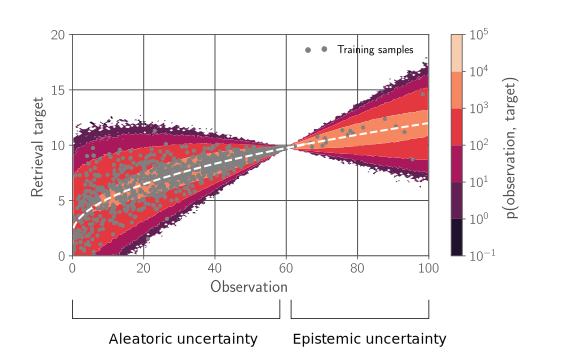
\includegraphics[width=\textwidth]{uncertainties}
  \caption{
    Illustration of aleatoric and epistemic uncertainty. The graph
    displays the relationship between observations and retrieval target
    for a hypothetical retrieval scenario. In the left part of graph the
    uncertainties are dominated by aleatoric uncertainty, whereas in
    the right part they are dominated by epistemic uncertainty.
  }
  \label{fig:machine_learning:uncertainties}
\end{figure}

The final source of uncertainty is caused by differences between the training
data and the data that the model is actually applied on. It is typically
referred to as \textit{covariate shift}. It is obvious that when the wrong data
is used to train the model, it is likely to produce wrong results. However,
subtle changes between training data and the actual data that the model is
applied on are not uncommon and can  increase the predictive uncertainty of
the model.

\subsection{Revisiting the precipitation retrieval}

To provide a demonstration of the capabilities of the deep learning methods,
Fig.~\ref{fig:machine_learning:retrieval_comparison} revisits
the retrieval example introduced above and displays the results from two additional
retrievals, which have been trained using the same data.

The first one is based on an MLP, which uses the same single-pixel input as the
linear regression model. The results from this retrieval are shown in panel (b).
Compared to the reference precipitation shown in panel (d), the results show
modest improvements in the structure of the precipitation, but its spatial
extent is still strongly overestimated. Since the MLP uses only information from
a single input channel, it is severely limited in the relations that it can
learn. It is therefore not surprising that it does not work much better than the
linear regression model.

To explore the full potential of deep learning methods, the second model uses a
CNN to retrieve precipitation using the full input image and all 16 channels of
the geostationary observations simultaneously. These results show clear
improvements both in the structure of the retrieved precipitation as well as its
spatial extent.

\begin{figure}
  \centering
\includegraphics[width=\textwidth]{retrieval_comparison}
\caption{Retrieved precipitation from a linear regression model
  (panel (a)), an MLP applied separately to each input pixel
  (panel (b)) and a CNN that predicts precipitation for the
  full input image using all available channels (panel (c)).
  The reference precipitation measured by the combined radar
  and passive microwave retrievals of the GPM core observatory
  are shown in panel (d).}
\label{fig:machine_learning:retrieval_comparison}
\end{figure}

This example clearly demonstrates the ability of deep learning techniques to
improve remote sensing retrievals. However, it should also be noted that the
computational effort required to train these models increases by orders of
magnitude. The simple linear regression model used here takes at most a few
seconds to train. The training of the MLP and CNN models, on the other hand,
takes hours respectively days and uses dedicated computing hardware. This is in
general not an issue because the training is a one-time effort and the
evaluation of the model is much faster, but nonetheless a fact that deserves
consideration.

The results in Fig.~\ref{fig:machine_learning:retrieval_comparison} show that
even the more advanced retrieval model fails to truthfully reproduce the
precipitation in the reference data. Since VIS and IR observations from
geostationary satellites are only sensitive to the upper parts of the clouds,
the inputs provided to the retrieval are only indirectly related to
precipitation at the surface. The ill-posed character of the retrieval problem
dictates that any specific prediction from a neural network will be wrong. Given
this fundamental nature of remote sensing retrievals, the next section explores
how neural networks can learn how wrong they expect to be.


\section{Handling uncertainty in remote sensing retrievals}

One of the issues that this thesis aims to address is the quantification of
retrieval uncertainties in machine-learning-based remote sensing retrievals. The
two methods that were explored in the appended studies fall into the category of
probabilistic regression methods. This means that they account for the aleatoric
uncertainty in the prediction but neglect epistemic uncertainty and covariate
shift. Below, these two approaches are presented followed by a discussion of
other approaches for quantifying uncertainties in neural network predictions.

\subsection{Probabilistic regression}

Aleatoric uncertainty arises due to ambiguous samples in the training data. The
fact that these ambiguities are represented in the training data means that they
can be predicted by a suitably trained neural network model. To allow for this,
the deterministic formulation of regression, i.e. to predict a single value $y =
f(\vec{x})$, is replaced by a probabilistic formulation, which aims predict the
probability distribution $p(y|\vec{x})$ of $y$ given the input vector $\vec{x}$.

\subsubsection{Quantile regression neural networks}

%To predict a distribution $p(y|x)$ the neural network model can trained
%to predict parameters of a parametrized probability distribution and
%an optimization criterion for the training can be obtained by maximizing the
%likelihood of the training samples under the predicted distribution. Assuming
%$p(y|x)$ to be Gaussian distributed with mean $\mu = f(x)$ and constant standard
%deviation yields a training criterion equivalent to the MSE loss.

Quantile regression neural networks (QRNNs) predict the distribution
$p(y|\vec{x})$ for a scalar output $y$ using a sequence of its quantiles. Given
a fraction $\tau \in [0, 1]$, the corresponding quantile $y_\tau$ is defined as
\begin{align}
  y_\tau &= F^{-1}(\tau)
\end{align}
with $F(y) = \int_{-\infty}^y p(y|\vec{x})\ dy$ the cumulative distribution
function (CDF) of the distribution $p(y|\vec{x})$. A neural network can learn to predict a quantile
$y_\tau$ by training it to minimize the quantile loss
\begin{align}
  \mathcal{L}(y_\tau, y) &=
  \begin{cases}
    \tau  |y_\tau - y| & \text{if } y > y_\tau \\
    (1 - \tau)  |y_\tau - y| & \text{otherwise} \\
    \end{cases}
\end{align}
where $y_\tau$ is the predicted quantile and $y$ is the reference output value
from the training data. It is important to realize here  that $y$ is only
required to be an ordinary sample of the distribution $p(y|\vec{x})$ and does not
require the distribution $p(y|\vec{x})$ to be explicitly represented in the
training data.

The approach can be extended to the prediction of multiple quantiles
corresponding to a sequence of quantile fractions $\mathrm{T} = \{\tau_1,
\ldots, \tau_N\}$ by training the network to minimize the sum of the quantile
losses
\begin{align}
  \mathcal{L}_\mathrm{T}(\vec{y}_T, y) &= 
  \sum_{\tau \in \mathrm{T}} \mathcal{L}_\tau(y_\tau, y)
\end{align}
where now $\vec{y}_T = [y_{\tau_1}, \ldots, y_{\tau_N}]$ is a vector of predicted quantiles.

The basic principle of QRNNs is illustrated
Fig.~\ref{fig:machine_learning:qrnn}. To predict the distribution of a scalar
variable $y$ conditioned on a vector of inputs $\vec{x}$, QRNNs use a neural
network to transform the vector of inputs into a vector of outputs. The outputs
correspond to a sequence of quantiles, which can be used to derive a piece-wise
linear approximation of the CDF of $p(y|\vec{x})$.

\begin{figure}[btp]
  \centering
  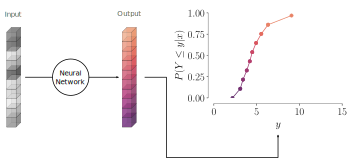
\includegraphics[width=.75\textwidth]{qrnn.pdf}
  \caption{Basic principle of QRNNS. QRNNs predict the distribution of
    a scalar output variable $y$ using a vector of quantiles from which the
    an approximation of the CDF of the distribution can be constructed.}
  \label{fig:machine_learning:qrnn}
\end{figure}

Using quantiles to represent the distribution $p(y|\vec{x})$ has the advantage
that the neural network can learn the shape of the posterior distribution of the
retrieval. This is in contrast to other probabilistic regression methods, which
often impose a more constrained parametrized form of $p(y|x)$, such as a Gaussian
whose mean and standard deviation are predicted.

An unresolved issue with QRNNs is quantile crossing. There is nothing that
ensures that the quantiles predicted by a QRNN as they are employed here are in
increasing order. QRNNs can thus produce mathematically inconsistent
predictions, where quantiles of lower fractions exceed those of higher
fractions. However, at least for the applications considered in this thesis,
this was not found to be a critical issue.

\subsubsection{Density regression neural networks}

The second approach for predicting the distribution $p(y|\vec{x})$ is based on
the work by \citet{oord16} and \citet{sonderby20}. Since it has not been given
an explicit name by the authors, it is referred to here as density regression
neural networks (DRNNs). In this approach, the regression problem is cast as a
classification problem by discretizing the domain of output values $y$ into bins
$y_0, \ldots, y_n$ and then predicting for each bin the probability $p_i(y >=
y_{i - 1}, y < y_i)$ of the observed $y$ falling into the $i$th bin.

Mathematically this is implemented by minimizing the
categorical cross-entropy loss
\begin{align}
  \mathcal{L}(\hat{\vec{p}}, y) &=  -\log(\hat{p}_i) \text { with i such that } y_{i - 1} \leq y < y_i.
\end{align}
where $\hat{\vec{p}} = [\hat{p}_1, \ldots, \hat{p}_n]$ is a vector of predicted probabilities.

The predicted vector of bin probabilities can then be used as a piece-wise
constant approximation of the PDF of $p(y | \vec{x})$, as illustrated in
Fig.~\ref{fig:machine_learning:drnn}. Since the CDF of $p(y | \vec{x})$ can be
calculated from the PDF and vise versa, QRNNs and DRNNs are functionally very
similar. Compared to QRNNs, DRNNs have the advantage of avoiding quantile
crossing by construction. What may be a disadvantage of DRNNs is that they require
a relatively high number of outputs  when the values of $y$ vary across a wide
range.
\begin{figure}[btp]
  \centering
  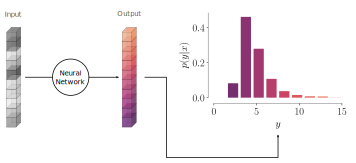
\includegraphics[width=.75\textwidth]{drnn.pdf}
  \caption{The basic functioning of QRNNS. QRNNs predict the distribution of
    a scalar output variable $y$ using a vector of quantiles from which the
    an approximation of the CDF of the distribution can be constructed.}
  \label{fig:machine_learning:drnn}
\end{figure}

\subsubsection{The aleatoric approximation}

Both QRNNs and DRNNs only learn to quantify the aleatoric uncertainty and
neglect epistemic uncertainty and covariate shift. It is thus necessary that the
aleatoric component of the predictive uncertainty dominates the two other types
of uncertainties for these models to produce reliable uncertainty estimates.
Given that remote sensing observations are produced in a controlled environment
and the range of possible observations is generally well understood, it is
usually possible to obtain large amounts of reliable training data, which
minimizes epistemic uncertainty and the effects of covariate shift. Given the
cost of designing and operating these observation systems, one should expect
that an effort is made to minimize both epistemic uncertainty and covariate
shift, thus leaving the aleatoric uncertainty as the only irreducible source of
uncertainty in the measurements. Additional, empirical evidence for the
usefulness of the aleatoric approximation comes from the results presented in
this thesis, where the probabilistic predictions from QRNNs and DRNNs were found
to provide reliable estimates of the retrieval uncertainty.

\subsubsection{Further limitations}

A further limitation of QRNNs and DRNNs is their handling of multiple retrieval
outputs. The formulations presented above were based on the assumption of a
scalar retrieval output $y$. These approaches can easily be extended to multiple
output variables by simply minimizing the mean of their individual losses. This
was found to work well in practice but provides no way of representing the
correlations between the multiple outputs in the results. QRNNs and DRNNs are
therefore not able to produce random samples  that accurately the correlations
between the output variables.

\subsection{Other approaches for quantifying uncertainties}

Because of their limitations, QRNNs and DRNNs may not be the best choice for all
applications. Therefore, the following section briefly reviews other approaches
for quantifying retrieval uncertainty and compares them to the probabilistic
regression approach.

\subsubsection{Bayesian neural networks}

Bayesian neural networks (BNNs) can handle both epistemic and aleatoric
uncertainty. For BNNs, not only the target $y$ is assumed to be a random
variable, but also the parameters $\vec{\theta}$ of the neural network model. The
random distribution of these parameters represents the uncertainty caused by the
limited amount of training data that the model is trained on. Instead of
learning specific parameters, a BNN learns a distribution of each of its
parameters.

A single prediction from a BNN $p(y|\vec{x}, \vec{\theta})$ for a specific input
$\vec{x}$ is obtained by sampling values of the model parameters from the learned
distributions and using them to evaluate the model. The epistemic uncertainty in
the model predictions is typically quantified by sampling multiple instances of
the model parameters $\vec{\theta}$ and evaluating the model for each of them. For
inputs $\vec{x}$ that the model has encountered often during training, the
distribution of $\vec{\theta}$ values will be sharp so that the distribution
$p(y|\vec{x}, \vec{\theta})$ does not change much for different realizations
of the model parameters $\vec{\theta}$. For
samples where this is not the case, there will be a larger spread and thus
higher epistemic uncertainty in the predictions.

Despite their ability to quantify both aleatoric and epistemic uncertainty, BNNs
have not yet found widespread adoption in practical applications. One reason for
this is likely that their training takes significantly more time. Another
disadvantage is that the quantification of epistemic uncertainty requires
evaluating the network multiple times. This typically increases the time
required to evaluate the model by an order of magnitude, which is a
disadvantage for applications that require high throughput.

Despite these potential disadvantages, \citet{orescanin22} have recently
demonstrated the application of Bayesian neural networks to the classification
of precipitation types and shown that the predicted uncertainties are
well-calibrated. They also found that the predictive uncertainty is dominated by
aleatoric uncertainty, which provides further evidence for the validity of
the aleatoric approximation.

\subsubsection{Generative models}

Generative models are another approach for quantifying uncertainties in neural
network predictions. Instead of predicting the conditional probability
distribution $p(\vec{y}|\vec{x})$ explicitly, these methods are trained to generate
samples from the distribution directly. These methods have gained popularity in
computer vision tasks due to their ability to generate samples from highly
complex probability distributions such as images of faces or generic objects.

The advantage of this approach is that it can handle spatial correlations in the
uncertainties, which is not the case for the other methods discussed so far.
This means that they can produce spatially coherent samples of the retrieved
variables that look very realistic. Recent work has explored the application of
generative models for short-term weather forecasting \citep{ravuri21} and
probabilistic downscaling of precipitation \citep{harris22, leinonen20}.
However, these models are also known to be more difficult and take longer to
train. In addition to that, they also need to be evaluated multiple times to
calculate statistics of the posterior distribution, which increases the
computational requirements of the retrieval.


\chapter{Contributions}

The previous chapter introduced QRNNs and DRNNs as machine-learning based
methods to perform remote sensing retrievals. The motivation for this was to
find a practical approach to combine the expressiveness of modern, deep neural
networks with the theoretically sound handling of uncertainties of conventional
inverse-theory-based retrieval methods. To explore the validity and
practicality of the proposed methods we have tested them using idealized
scenarios and developed multiple real-world retrieval applications. This section
presents this work and summarizes the main results.

\section{Handling retrieval uncertainty with neural networks}

The first of the append papers, titled \textit{A neural network approach to
estimating a posteriori distributions of Bayesian retrieval problems} and
published in \citet{pfreundschuh18},} proposes the use of QRNNs for remote
sensing retrievals. The motivation for this study were the shortcomings the
retrieval methods that were available at the time of its writing. The Bayesian
framework provides a principled way of handling the retrieval uncertainties
(see Sec.~\ref{sec:machine_learning:retrieval_problem}), but the commonly used
methods are computationally complex. While retrievals based on neural networks
were already common and often offered superior performance  in terms of
computational cost as well as accuracy, they typically neglected retrieval
uncertainties.

The aims of the study were two-fold: (1) To demonstrate the compatibility of
QRNNs with conventional Bayesian retrieval methods and (2) to demonstrate the
practicality of QRNNs by applying them to a real-world retrieval application.

To demonstrate the compatibility of QRNNs with conventional Bayesian retrieval
methods, we made use of an idealized but realistic retrieval scenario, in which
the true Bayesian solution could be calculated to arbitrary precision. We then
used QRNNs and Bayesian Monte Carlo Integration (BMCI), a commonly used Bayesian
retrieval method, to solve the retrieval and compared the solutions to the true
solution. BMCI calculates an approximate solution of the retrieval problem using
a database of observations and corresponding reference values. This makes it
similar in this regard to a machine learning method. We found that QRNNs work at
least as good as BMCI in solving the retrieval problem when both are based on a
sufficiently large dataset. For smaller datasets, there was a clearer advantage
for QRNNs indicating that they cope better with the curse of dimensionality.

This first result has two important implications. Firstly, it showed that QRNNs
can be used instead of BMCI and expected to work at least as good given the same
training data. Even if the advantage of neural networks over BMCI on the
considered dataset was marginal when sufficient training data is available, the
use of neural networks offers distinct advantages. For one, the time required to
produce a neural network prediction is independent of the training data size.
This is not the case for BMCI, for which this time scales linearly with the size
of the training database. This means that the amount data that can be used by
the method may be limited by operational processing requirements. Besides that,
because of the flexibility of QRNNs they can be easily extended to image or time
series data, which is again not the case for BMCI. The second important
implication of these results was that it showed the compatibility of
probabilistic machine learning methods with the Bayesian retrieval methods.
These results link the extensive theory on Bayesian retrieval methods
\citep{rodgers00, tarantola05} with and machine-learning-based retrieval
methods. The correspondence between the training data of the neural network and
the a priori distribution of a Bayesian retrieval, highlights the role the a
priori distribution plays for the retrieval results and accurate quantification
of retrieval uncertainties.


%Two experiments were performed in the study. The first one used an idealized
%retrieval scenario in which samples from the posterior distribution $p(y|x)$
%could be calculated using Markov Chain Monte Carlo (MCMC) methods. MCMC is
%generally too slow to be used in operational processing, but its ability to
%generate samples from the true posterior distribution makes it suitable to
%provide a reference solution against which QRNNs and another Bayesian retrieval
%method could be evaluated. A principal results from this experiment is shown
%Fig.~\ref{fig:contributions:cdfs_qrnn_bmci}. The plot displays the retrieved
%CDFs of the posterior distributions using QRNN and Bayesian Monte Carlo
%Integration (BMCI), which is a commonly used Bayesian retrieval methods. Each
%panel shows the reference CDF obtained using MCMC in the background and the CDFs
%obtained using BMCI in blue, those obtained from a single QRNN using a solid red
%line and those obtained from an ensemble of QRNNs using red markers. The shown
%samples were chosen according to the Kolmogorov-Smirnov of the BMCI
%($\text{KS}_\text{BMCI}$) and QRNN ($\text{KS}_\text{QRNN}$), which measures
%the agreement between the reference and retrieved CDF, and thus show retrieval
%results of varying quality from each retrieval.
%
%The main finding from this first experiment is that the CDFs retrieved using
%QRNN and BMCI agree very well with the reference CDF calculated using MCMC. This
%indicates that probabilistic neural network retrievals are consistent with the
%Bayesian solution of inverse problems with the a priori distribution being
%represented by the training data.
%
%\begin{figure}
%  \centering
%  \includegraphics[width=\textwidth]{cdfs_qrnn_bmci}
%  \caption{ Retrieved a posteriori CDFs obtained using MCMC (gray), BMCI (blue),
%    a single QRNN (red line) and an ensemble of QRNNs (red marker). Cases
%    displayed in the first row correspond to the 1st, 50th, 90th and 99th
%    percentiles of the distribution of the Kolmogorov– Smirnov statistic of BMCI
%    compared to the MCMC reference. The second row displays the same percentiles
%    of the distribution of the Kolmogorov–Smirnov statistic of the single-QRNN
%    predictions compared to MCMC.}
%  \label{fig:contributions:cdfs_qrnn_bmci}
%\end{figure}

The second experiment from this study applied QRNNs to the retrieval of cloud
top pressure (CTP) from infrared observations from the Moderate Resolution
Imaging Spectroradiometer (MODIS). Comparison of the QRNN retrieval to an
existing retrieval using a deterministic neural network showed that QRNNs yield
comparable or better accuracy for point predictions with the added benefit of
providing reliable uncertainty estimates. In particular, we show the ability of
the QRNN to represent non-Gaussian retrieval errors and the superiority over
commonly assumed Gaussian error models. A consequence of these findings was the
adoption of QRNNs for the operational production of near real-time retrievals of
cloud top pressure at the European Organisation for the Exploitation of
Meteorological Satellites.

\section{Passive microwave precipitation retrievals}

The second study included in thesis, titled \texti{%
GPROF-NN: A neural network based implementation of the Goddard Profiling Algorithm %
} and published as \citet{pfreundschuh22a}, applied the QRNN methodology to
the retrieval of precipitation from PMW observations of the GPM mission.
GPM  is an international satellite mission lead by NASA and JAXA, which aims
to provide global measurements of precipitation at high spatial and temporal
resolution. The mission is built around the Core Observatory satellite, which
carries a precipitation radar and a PMW sensor dedicated to
the remote sensing of precipitation. Retrievals from the combined radar/PMW
observations from the Core Observatory are used to build a retrieval
database that is in turn used to for the retrievals of a constellation 
PMW sensors. As of this writing, the GPM constellation comprises 9 active
satellites.

The algorithm that is used to retrieve precipitation from GMI, the PMW sensor on
the Core Obsevatory, and the other PMW sensors of the GPM constellation is the
Goddard Profiling Algorithm (GPROF, \citeauthor{kummerow15},
\citeyear{kummerow15}). GPROF is based on the BMCI method and retrieves surface
precipitation as well as profiles of hydrometeor concentrations and latent
heating rates. The aim of the study was to assess the potential benefits of
replacing BMCI with a neural network based retrieval. Besides that, the study
aimed to explore to what extent the accuracy of the retrieval can be improved if
structural information from neighboring pixels is incorporated into the
retrieval instead of processing each pixel separately as the current
implementation does. To this end, two neural network based implementation were
developed. The first one, named GPROF-NN 1D, uses an MLP to retrieve
precipitation from a single pixel. The second one, GPROF-NN 3D, uses a CNN to
retrieve precipitation across the full swath simultaneously. This allows the
retrieval to leverage structural information in the observations, which is not
available to the two other implementations.

Both the GPROF-NN 1D and GPROF-NN 3D retrieval were developed to be functionally
equivalent to the currently operational GPROF algorithm so that they can
potentially replace it in an upcoming update. Moreover, the implementations were
restricted to use exactly the same data for their training as the current method
to ensure that the comparison of the three methods only reveals differences
between the retrieval methods. This required the development of a training
pipeline that can be applied to all sensors of the GPM constellation.

While the application of QRNNs to the GPROF algorithm is straight-forward from a
theoretical perspective, the requirements of developing a retrieval that uses
identical input data, produces equivalent outputs and uses the same data as the
current implementation of GPROF proved challenging. The training data for the
sensors of the GPM constellation makes use of radiative transfer simulation,
however these are generated not for full satellite swaths of observations but
only for single pixels this made the raw training data unsuitable for the
training of a CNN. Since extending the simulations to the full swath is
currently not possible, we trained an intermediate CNN-based 'retrieval' to
emulate the simulation of PMW observations.

%proved challenging especially for the GPROF-NN 3D retrieval. The training data
%for all sensors of the GPM constellation is based on combined radar/radiometer
%observations from the GPM satellite. Since these observations are only available
%at a $\SI{100}{\kilo \meter}$-wide swath at the center of the GMI observations,
%a way had to be found to extent these to the full GMI-swath and to remap them to
%the viewing geometries of the other sensors. The current approach uses an
%intermediate simulator network to extend the simulated observations to the full
%swath of GMI, which are then remapped to the viewing geometries of other sensors
%by interpolation. This solution should be a considered a heuristic that was
%pursued mainly because extending the simulations that are routinely performed
%for the generation of the GPROF training data would have been outside the scope
%of this study.

The main results from this study are estimates of potential improvements in
retrieval accuracy that can be realized by upgrading GPROF to either the
GPROF-NN 1D or GPROF-NN 3D retrieval. We found consistent improvements for the
GPROF-NN 1D algorithms across a range of accuracy metrics and across all
retrieved quantities. The accuracy is improved further by the GPROF-NN 3D
retrieval, which yields improvements similar in magnitude to those provided by
the GPROF-NN 1D algorithm of the GPROF baseline retrieval. Furthremore, we found
that the effective resolution of the retrieval improves by at least
$\SI{40}{\percent}$ with the neural network based retrieval. The study included
results from two case studies of Hurricane overpasses from the GMI and MHS
sensors, which provided limited evidence that the retrieval improvements can be
expected to carry over to real observations.

Although the results from this study were promising, their significance was
limited because the evaluation of the retrieval was limited to the same source
of data, which was used for the generation of the training data. Since the
objective of the study was to compare the BMCI retrieval method and QRNNs, this
simplification was justified because in an validation against independent data,
the benefits of the neural-network-based retrieval may have been masked by
deviations of the training data from the validation data. However, the
practically more relevant question was to what extent do these improvements
carry over to comparison against independent validation data.

We aim to address this question in a study that is currently under preparation
and included in this thesis as the third paper, titled \texit{% Evolution of the
GPROF passive microwave precipitation retrievals evaluated against ground
radar measurements over the continental US and the Pacific Ocean% }. Since the
development of the GPROF-NN algorithms was performed in parallel with a new
version of the GPROF retrieval, this study aimed to assess improvements in
this new version of GPROF (GPROF V7) against the previous version (GPROF V5)
and assess the potential benefits of replacing GPROF with GPROF-NN 1D or 3D in
a future update. Furthermore, the study aims to identify  potential outstanding issues
impeding the adaptation of the GPROF-NN retrievals to operational processing.

The validation is based on ground-radar measurements of precipitation
specifically created for the validation of GPM measurements. It is
based measurements from the continental United States (CONUS) and a ground radar
station on the Kwajalein atoll in the Pacific Ocean to complement the primarily
land-based observations over CONUS with observations over ocean.

The main focus of this study are retrievals from the GMI radiometer, which plays
a special role in the GPM constellation due to it placement on the Core
Observatory together with the precipiation radar and it being designed
specifically for the retrieval of precipitation. The accuracy of the
precipitation retrieved from the GMI sensor using the two version of the
conventional GPROF algorithm as well as the two GPROF-NN is evaluated for two
years of co-locations. The results clearly show that the benefits of the
neural-network-based implementation of GPROF carry over to validation against
independent precipitation measurements. In particular, we find that the
effective resolution of the retrieved precipitation improves by more than
a factor of 2 over land.

In addition to GMI, we also investigated the retrieval accuracy other sensors of
the GPM constallation using one year of observations over the CONUS as the
training for these sensors is completed. For the two sensors that we have
assessed we also find improvements in retrieval accuracy. This is an encouraging
result because the training for them is derived from simulated observations,
while it is derived from real observations for GMI.


\section{VIS/IR precipitation retrievals}

While the neural-network-based implementation of GPROF provided clear evidence
for the potential of neural-network based precipitation retrievals, the
constraint of a retrieval that provides the same output as the currently
operational GPROF algorithm limited the exploration of retrieval improvements to
currently available retrieval outputs. The assessments presented in
\citet{pfreundschuh22} and \citet{pfreundschuh22c} therefore focused mostly on
deterministic precipitation estimates and thus did not explore the full
potential of the probabilistic predictions afforded by the neural network.

The aim of the study presented in \citet{pfreundschuh22b} was to explore the
full potential of probabilistic neural-network based precipitation retrievals in
the context of near real-time retrievals from VIS/IR observations over Brazil.
The input data for the retrieval comes from the advanced baseline imager (ABI)
on the geostationary operational environmental satellite (GOES) 16. To train the
retrieval, the input observation were co-located with combined radar-radiometer
measurements from the GPM core observatory satellite.

To validate the retrieval its results were compared to 1 month of gauge
measurements. The retrieval accuracy was assessed by comparing it to the
retrieval algorithm that is currently used operationally at the Brazilian
institute of space research as well as to commonly used global precipitation
retrievals. We were able to show that, despite the limited information content
of VIS/IR observations, deep-learning-based retrievals outperform currently
available methods, even those that merge IR observations from geostationary
satellite with PMW observations polar-orbiting platforms.

Furthermore, the study explored the potential of the probabilistic precipitation
estimates. We were able to show that, after correcting for differences in the
precipitation statistics of the training data and gauge measurements, confidence
intervals derived from the probabilistic predictions were well calibrated
against the gauge measurements. We also provided results that the probabilistic
predictions improve the detection of heavy precipitation.


\section{Cloud correction for data assimilation}

The final study included in this thesis explores the application of QRNNs to
remove the effect of clouds from microwave observations. The observations
contain important information on the distribution water vapor in the atmosphere
and are used in data assimilation systems to find good initial conditions for
numerical weather forecasts. However, the presence of hydrometeors in the
atmosphere makes radiative transfer calculation much more complex which
complicates the use of observations. Since the information on the hydrometeors
themselves is not really used in the data assimilation system, a model that
could accurately predict how these observations would look when the effect of
the hydrometeors was removed, would allow these observations to in a less
complex and computationally more efficient way.

Because of their impact on the radiative transfer, operational data assimilation
systems have to detect observations that are affected by clouds to either
correctly handle them if the DA system is sufficiently advanced to handle cloudy
observations or to discard them altogether. The first experiment therefore
assessed the potential of applying QRNN to correct cloud-contaminated
observations from an existing sensor and compared the performance to existing
methods. The experiment showed that the QRNN-derived correction leads to a lower
bias in the observations than the residual biases in currently used filtering
methods, which reject up to $\SI{30}{\percent}$. The important point here is that the QRNN-based
cloud correction achieves this without rejecting any observations, which would
makes more observations available to the data assimilation system.

The second experiment then extended the approach to a soon-to-be-launched and
and a hypothetical satellite sensor. Both of the will carry microwave sensors
with channels above $\SI{300}{\giga \hertz}$. These high frequencies make the
observations more sensible to scattering from ice particles, which further
complicates their use in data assimilation. In these cases QRNN-based cloud
correction would provide a simple alternative to ingesting this information into
data assimilation systems by using the hydrometeor information afforded by the
high-frequency channels to improve the removal of cloud contamination at lower
frequency channels. The results show that channels at frequencies exceeding
$\SI{300}{\giga \hertz}$ are well suited for cloud correction.

This study proposed a novel application of QRNNs for the correction of microwave
observations for use in data assimilation and retrievals of water vapor
profiles. QRNN-based cloud correction provides superior performance to existing
methods. In addition to that, the predicted uncertainties provide more accurate
error estimates than currently used error models for data assimilation.
Finally, the simulation-based assessment of the potential of microwave observations
at sub-millimeter wavelength lead to the selection of these channels for an
upcoming satellite mission \citep{arctic_weather_satellite}.

\section{Future work}

The findings of this thesis suggests several directions of future research.
These will be discussed below.

\subsection{Handling retrieval uncertainty with neural networks}

This thesis has proposed and assessed to neural-network-based methods for
handling uncertainties in remote sensing retrievals and shown their practicality
across multiple retrieval applications. The advantage of these methods is
certainly their simplicity. Only a minor modification in the training process is
required to migrate a deterministic neural network retrieval to a probabilistic
one.

There are, however, two important limitations of the approaches: Their
incapability of handling correlations in the retrieval outputs and their
reliance on the aleatoric assumption, which postulates that the predictive
uncertainty is dominated by the aleatoric uncertainty.

It would therefore be valuable to systematically evaluate the approaches against
Bayesian neural networks and generative model on a set of atmospheric retrieval
problems. In particular, it would be important to evaluate the methods not only
with respect to retrieval accuracy but to also take into account the effect on
downstream applications of the data. This would provide guidance in what scenarios
the computationally more complex alternative approaches should be applied.

\subsection{GPM precipitation retrievals}

Due to the good performance of the developed GPROF-NN retrievals, they are being
considered for operational implementation for the PMW precipitation retrieval of
the GPM mission. This will require some additional investigations regarding the
climatological stability of the GPROF-NN retrievals across different satellites.

In addition to that, the migration to a neural-network-based implementation
opens up for a number of improvements of the GPROF retrieval. One of them is the
extension of the training data to cover multiple years of observations. As was
found in \citep{pfreundschuh22c}, this may improve the climatic stability of the
retrieval. Furthermore, including samples from the posterior distribution may
improve the representation of extreme precipitation in the retrieval results,
which is relevant for climatological studies.

\subsection{VIS/IR precipitation retrievals}

The results presented in \citet{pfreundschuh22b} clearly showed the
potential of deep neural networks for precipitation retrieval from
geostationary satellites. According to personal communication, the
developed retrieval is also considered for operational application.

An interesting result that emerged from this study was that, despite the low
information content of the geostationary observations on precipitation,
deep-learning-based retrievals can outperform highly complex retrieval pipelines
which integrate observations from multiple sensors. This indicates that the use
of information in multi-sensor retrievals is sub-optimal. In a future project,
we will therefore explore the potential of fusing observations from different
sensors directly using a single neural network.


\bibliographystyle{plainnat}
\bibliography{references} 

\part{Appended papers}

\renewcommand{\chaptername}{Paper}
\setcounter{chapter}{0}

\chapter{A neural network approach to estimating a posteriori distributions of Bayesian retrieval problems} 
\chaptermark{Neural networks for Bayesian retrieval problems}            % Short title for the page header
\label{chap:qrnn}
\thispagestyle{empty}
\cleardoublepage            % skip back side of the page
\includepdf[pages=-]{papers/amt-11-4627-2018}

\chapter{GPROF-NN: A neural network based implementation of the Goddard Profiling Algorithm} 
\chaptermark{GPROF-NN}
\label{chap:qrnn}
\thispagestyle{empty}       % no page numbers
\cleardoublepage            % skip back side of the page
\includepdf[pages=-]{papers/gprof_nn_manuscript}

\chapter{An improved near-real time precipitation retrieval for Brazil} 
\chaptermark{Near-real time precipitation retrieval for Brazil}
\thispagestyle{empty}       % no page numbers
\cleardoublepage            % skip back side of the page
\includepdf[pages=-]{papers/manuscript}

\chapter{Can machine learning correct microwave humidity radiances for the influence of clouds?} 
\chaptermark{Correcting microwave humidity radiances for the influence of clouds}
\thispagestyle{empty}       % no page numbers
\cleardoublepage            % skip back side of the page
\includepdf[pages=-]{papers/amt-14-2957-2021}

\end{document}
